\documentclass{article}
\usepackage[letterpaper,top=2cm,bottom=2.5cm,left=3cm,right=3cm,marginparwidth=1.75cm]{geometry}
\usepackage[round]{natbib}
\usepackage{amsmath,amssymb,amsfonts}%
\usepackage{geometry}%
\usepackage{color}
\usepackage{graphicx}
\usepackage{authblk}
\usepackage{nameref}
\usepackage[right]{lineno}
\usepackage{subcaption}
\usepackage{tikz}
\usetikzlibrary{math,calc,positioning}
\usepackage{url}
\usepackage[symbol]{footmisc}
\usepackage[hidelinks]{hyperref}

\newcommand{\noderef}[1]{\textsf{#1}}
\newcommand{\tsinfer}[0]{\texttt{tsinfer}}
\newcommand{\kwarg}[0]{\texttt{KwARG}}
\newcommand{\argweaver}[0]{\texttt{ARGweaver}}
\newcommand{\argweaverD}[0]{\texttt{ARGweaver-D}}
\newcommand{\relate}[0]{\texttt{Relate}}
\newcommand{\espalier}[0]{\texttt{Espalier}}
\newcommand{\arbores}[0]{\texttt{Arbores}}

\begin{document}


\title{\vspace{-1.5em} \bf
A general and efficient representation of ancestral recombination graphs}

\author[1]{Yan~Wong}
\author[2,3$\star$]{Anastasia~Ignatieva}
\author[4,5$\star$]{Jere~Koskela}
\author[6]{Gregor~Gorjanc}
\author[7,8]{Anthony~W.~Wohns}
\author[1$\dagger$]{Jerome~Kelleher}
\affil[ ]{\mbox{}\vspace{-2.5em}}

\maketitle

\setlength{\skip\footins}{1em}
\setlength{\footnotemargin}{0.5em}
\renewcommand{\thefootnote}{\arabic{footnote}}
\footnotetext[1]{Big Data Institute, Li Ka Shing Centre for Health
Information and Discovery, University of Oxford, UK}
\footnotetext[2]{School of Mathematics and Statistics, University of Glasgow, UK}
\footnotetext[3]{Department of Statistics, University of Oxford, UK}
\footnotetext[4]{School of Mathematics, Statistics and Physics, Newcastle University, UK}
\footnotetext[5]{Department of Statistics, University of Warwick, UK}
\footnotetext[6]{The Roslin Institute and Royal (Dick) School of Veterinary Studies, University of Edinburgh, UK}
\footnotetext[7]{Broad Institute of MIT and Harvard, Cambridge, USA}
\footnotetext[8]{Department of Genetics, Stanford University School of Medicine, Stanford, USA}
\renewcommand{\thefootnote}{\fnsymbol{footnote}}
\footnotetext[1]{Joint second author, listed alphabetically}
\footnotetext[2]{Correspondence: jerome.kelleher@bdi.ox.ac.uk}

\vspace{-1em}

\begin{abstract}
As a result of recombination, adjacent nucleotides can have
different paths of genetic inheritance and therefore
the genealogical trees for
% surely saying nucleotides and "sample of sequences" is concrete enough
% here? This paper isn't for a general audience, let's just say what
% we're talking about in direct language understandable by population
% geneticists.
a sample of DNA sequences vary along the genome.
The structure capturing the details of these intricately interwoven paths of
inheritance is referred to as an ancestral recombination graph (ARG).
New developments have made it possible to infer ARGs at scale,
enabling many new applications in population and statistical genetics.
This rapid progress, however, has led to a
% Controversial, perhaps, but true?
substantial gap opening between theory and practice.
Standard mathematical formalisms,
% "detailing" here is intended to convey the we keep details about these
% events like recomb breakpoint.
based on exhaustively detailing the ``events'' that occur
in the history of a sample,
are insufficient to describe the outputs of current methods.
Moreover, we argue that the underlying assumption
that all events can be known and precisely estimated
is fundamentally unsuited to the realities
of modern, population-scale datasets.
We propose an alternative mathematical formulation that
encompasses the outputs of recent methods and
can capture the full richness of modern large-scale datasets.
By defining this ARG encoding in terms of
% we haven't define a "genome" yet, so need to give a bit of context
specific genomes and their intervals of genetic inheritance,
we avoid the need to exhaustively list (and estimate)
\emph{all} events. The effects of multiple events can be
aggregated in different ways, providing a natural way to express many
forms of approximate and partial knowledge about the
recombinant ancestry of a sample.
\end{abstract}

\textbf{Keywords:} Ancestral recombination graphs

\linenumbers
\section{Introduction}
\label{sec-intro}
% Para 1: ARGs are cool!
% NOTE: slight inaccuracy of "DNA" here offset by making the problem concrete.
Estimating the genetic genealogy of a set of DNA sequences
under the influence of recombination,
usually known as an Ancestral Recombination Graph (ARG), is a long-standing
goal in genetics.
Broadly speaking, an ARG describes the different paths of genetic inheritance
caused by recombination, encapsulating the resulting complex web of genetic
ancestry
(see \citet{lewanski2023era} for a biologically oriented introduction).
Recent breakthroughs
in large-scale inference
methods~\citep{rasmussen2014genome,kelleher2019inferring,speidel2019method,
schaefer2021ancestral,wohns2022unified,zhang2023biobank,zhan2023towards}
have raised the realistic prospect of ARG-based analysis becoming a standard part
of the population and statistical genetics toolkit~\citep{hejase2020summary}.
Applications using inferred ARGs as input have begun to
appear~\citep{osmond2021estimating,
fan2022genealogical,
hejase2022deep,
guo2022recombination,
zhang2023biobank,
nowbandegani2023extremely,
ignatieva2023distribution,
fan2023likelihood}
and many more are sure to
follow~\citep{harris2019database,harris2023using}.

% Para 2: What are they, though?
Although it is widely accepted that ARGs are important, there is some
confusion about what, precisely, an ARG \emph{is}.
% The grammar is a nightmare here - the stochastic process is singular, right?
In its original form,
developed by Griffiths and colleagues,
the ARG is an alternative
formulation of the coalescent with recombination~\citep{hudson1983properties},
where the stochastic process of coalescence and recombination
among ancestral lineages is formalised
as a graph~\citep{griffiths1991two,
ethier1990two,griffiths1996ancestral,griffiths1997ancestral}.
% Move into plural, an ARG is an instance of the data structure in this view
Subsequently, an ARG has come to be thought of as a data
structure~\citep{minichiello2006mapping}, i.e.\ describing
a \emph{realisation} of such a random process,
or an inferred ancestry of a sample of genomes.
The distinction between stochastic process
and data structure is not clear cut, however, and subfields use the term
differently (Appendix~\ref{sec-arg-history}).
Other subtly different concepts that we must be careful to distinguish
are the ``true'' ARG, % I don't see a better word for "true" here
describing the actual history of a sample of genomes,
and a ``population'' ARG which is
the true ARG of every individual in a population.
True ARGs are the underlying real history of a sample,
perfectly resolved into binary splits and mergers by
the cellular processes of meiosis and mitosis, regardless
of sampling density or population processes
(Appendix~\ref{sec-cell-lineages-and-args}).
Although population-scale true ARGs unquestionably exist,
they can also never be entirely known, in part because of a fundamental
lack of mutational information.
Even if mutation rate were high enough to uniquely identify every
recent branching point,
such a high rate would saturate the genome with mutations
and obscure deeper history.

% Population ARGs are here, now.
Population ARGs may seem fanciful, but the scale of
modern datasets makes it necessary for us to grapple with the idea.
The UK Biobank (UKB), for example, has
genotype data for around 500,000 humans~\citep{bycroft2018genome},
along with exome~\citep{backman2021exome} and
whole genome sequence~\citep{halldorsson2022sequences} data
for large subsets of the cohort.
UKB is just one of many such population-scale sequencing
projects~\citep[e.g.][]{turnbull2018hundred,
karczewski2020mutational,tanjo2021practical}.
Agricultural datasets are on a similar scale,
and also include dense multi-generational sampling
and near-perfect pedigree
information~\citep[e.g.][]{hayes20191000,Ros-Freixedes2020}.
Recent advances have made it possible to actually
\emph{estimate} ARGs at population scale:
ARGs have already been inferred for the 500,000
humans in UKB~\citep{kelleher2019inferring,zhang2023biobank}
and over a million SARS-CoV-2 genomes~\citep{zhan2023towards}.
While this new population-scale reality presents many
exciting opportunities, it also poses substantial challenges
to existing methodologies.

% What's the problem?
A major problem currently facing the field is that
classical mathematical formalisms and terminology
cannot adequately describe these vast inferred ARGs.
Fundamentally, these formalisms assume that an
ARG is known in complete detail
and are not suited to describing partial or approximate knowledge.
As we are actively inferring ARGs at the population scale,
and such ARGs can never be known in complete detail,
there is currently a substantial gap between our theoretical frameworks
and practical application.
The breakthroughs in scale achieved by recent
methods~\citep[e.g.][]{kelleher2019inferring,speidel2019method,zhang2023biobank}
are all based, in different ways, on inferring
approximate \emph{structures}
instead of a complete and fully detailed history.
% This is a digression from the maing point of the paragraph, so
% making it a parenthetical aside.
(Note that it is important to distinguish here between
structures and models: whether an inference method is based
on heuristics or a rigorous mathematical model is orthogonal
to the level of detail provided in its estimate.
One could heuristically estimate a fully precise ARG,
% this would be a cool thing to do!
or statistically sample a partial,
approximate ARG under a model
such as the coalescent.)
Although the term ``ARG'' is now often used in a general
sense~\citep[e.g.][]{mathieson2020ancestry,hejase2020summary,
schaefer2021ancestral,harris2023using,zhang2023biobank,fan2023likelihood},
informally
encompassing the varied approximate structures output by modern simulation and
inference methods~\citep{rasmussen2014genome, palamara2016argon, haller2018tree,
kelleher2019inferring, speidel2019method, baumdicker2021efficient,
zhang2023biobank},
there is no corresponding mathematical definition
that is sufficiently general.

We address this problem by providing a simple formal definition of an
ARG data structure, based on recording the intervals of
genetic inheritance between specific genomes.
We call this the ``genome ARG'', or gARG encoding. We
contrast this with the classical formal definition of an ARG, based on
recording common ancestor and recombination events, which we refer to as the
``event ARG'' or eARG encoding. We show that the new gARG encoding is a
substantial generalisation of the classical eARG approach,  providing much more
flexibility in how genetic inheritance can be represented, and encompasses the
outputs of modern methods. We show that the gARG approach can represent many
different types of approximation, in particular allowing us to systematically
describe uncertainty about the temporal ordering of multiple recombinations. It
is important to note that throughout we are interested in the details of these
competing mathematical formulations and their practical consequences.
% True ARGs, being perfectly resolved, can ultimately be described in
% either formalism

% This is nice to have, but probably won't work in the final version
% without section numbers. Let's deal with that when we get there I guess.
We begin in Section~\ref{sec-gARG} by providing a precise formal definition
of a gARG, illustrated by an example ARG embedded in pedigree.
We then provide a similar definition of the classical eARG
approach in Section~\ref{sec-eARG}, and consider its limitations
in the context of current datasets and research questions.
Following this, we discuss the important concept of ancestral material
in Section~\ref{sec-ancestral-material}, and how it relates
to the process of converting an eARG to a gARG.
We continue
in Section~\ref{sec-ARG-and-local-trees} by considering the relationship
between an ARG and its local trees. Contrary to the
prevailing view, we show that a suitably encoded sequence of local trees contains
precisely as much information as the corresponding ARG.
The gARG encoding opens a rich new set of details about ARGs,
including the ideas of locally unary nodes
(Section~\ref{sec-locally-unary-edges}),
the levels of detail that can be represented in an ARG
(Section~\ref{sec-ARG-simplification}),
and the degrees of precision about recombination
that can be stored and we may seek to infer (Section~\ref{sec-precision}).
These ideas have important practical considerations,
which we illustrate by examining the qualitative properties of
ARGs inferred by four recent methods for a classical benchmark
dataset in Section~\ref{sec-example-inferred-args}.
We then discuss how the gARG framework can be
efficiently implemented in Section~\ref{sec-efficiency},
and finish with an assessment of the key challenges facing
the field in the Discussion.
Finally, the literature on ARGs is large and
confusing, and we attempt to clarify some important aspects
in appendices, including
a brief history of ancestral graphs (Appendix~\ref{sec-arg-history}),
a description of the Big and Little ARG stochastic processes
 (Appendix~\ref{sec-big-and-little-arg}),
a survey of ARG inference methods (Appendix~\ref{sec-survey-arg-infer}),
and a discussion of ARGs at an individual vs cell
lineage level (Appendix~\ref{sec-cell-lineages-and-args}).

\section{Genome ARGs}
\label{sec-gARG}
We define a genome as the complete set of genetic material that a child
inherits from one parent. A diploid individual
% Q: will someone nitpick that we're assuming diploid obligate sexual species?
therefore carries two genomes, one inherited from each parent (we assume diploids here
for clarity, but the definitions apply to organisms of arbitrary ploidy).
We will also use the term ``genome'' in its
more common sense of ``the genome'' of a species,
and hope that the distinction will be clear from the context.
We are not concerned here with mutational processes or observed sequences,
but consider only processes of inheritance,
following the standard practice in coalescent theory.
We also do not consider structural variation, and assume that all
samples and ancestors share the same genome coordinate space.

A genome ARG (gARG) is a directed acyclic graph in which nodes represent
haploid genomes and edges represent
genetic inheritance between an ancestor and a descendant.
The topology of a gARG specifies that genetic inheritance
occurred between particular
ancestors and descendants, but the graph connectivity
does not tell us which \emph{parts} of their genomes were inherited.
In order to capture the effects of recombination
 we ``annotate'' the edges with the genome
coordinates over which inheritance occurred.
This is sufficient to describe the effects of inheritance under
any form of homologous recombination (such as multiple crossovers,
gene conversion events, and many forms of bacterial and viral recombination).

We can define a gARG formally as follows.
Let $N = \{1, \dots, n\}$ be the set of nodes representing
the genomes in the gARG,
and  $S \subseteq N$ be the set of sampled genomes.
Then, $E$ is the set of edges, where each element
is a tuple $(c, p, I)$ such that $c, p \in N$ are the child and
parent nodes and $I$ is the set of disjoint genomic intervals
over which genome $c$ inherits from $p$.
Thus, each topological connection between
a parent and child node in the graph is annotated with a set of
inheritance intervals $I$.
Here, the terms parent and child are used in the graph sense;
these nodes respectively represent ancestor and descendant genomes,
which can be separated by multiple generations.
We will use these two sets of terms interchangeably.

How nodes are interpreted, exactly, is application dependent.
Following \citet{hudson1983properties}, we can view nodes
as representing gametes, or we can imagine them representing
the genomes present in cells immediately before or after
some instantaneous event (Appendix~\ref{sec-cell-lineages-and-args}).
A node can represent any genome along a chain of cell divisions
or can be interpreted as representing one of the genomes of a
potentially long-lived individual. All these interpretations
are potentially useful, and equally valid under the assumptions
of the gARG encoding.
In many settings, nodes are dated, i.e.\ each
node $u\in N$ is associated with a time $\tau_u$,
and how we assign precise times will vary by application.
The topological ordering defined by the directed graph structure
and an arrow of time (telling us which direction is pastwards)
is sufficient for many applications, however,
and we assume node dates are not known here.
% This should be obvious, but seems like it needs to be said
In practical settings, we will wish to associate additional
metadata with nodes such as sample identifiers or quality-control metrics.
It is therefore best to think of the
integers used here in the definition of a node as an \emph{identifier},
with which arbitrary additional information can be associated.

\begin{figure}
\begin{center}
    \includegraphics[width=\textwidth]{illustrations/arg-in-pedigree}
\end{center}
\caption{\label{fig-arg-in-pedigree}
An example genome ARG (gARG) embedded in a pedigree.
(A) Diploid individuals (blue), visualised in a highly inbred pedigree and
labelled $D_1$ to $D_8$,
contain both paternal and maternal  genomes
labelled \noderef{a} to \noderef{p}. Black lines show inheritance paths connecting
genomes in the current generation (\noderef{a} to \noderef{d}) with their ancestors.
Genomes \noderef{a} and \noderef{c} are the product of two independent
meioses (recombination events, in red) between
the paternal genomes \noderef{e}
and \noderef{f}, and regions of genome inherited are shown with shaded colour.
Genomes are shaded such that where, backwards in time,
they merge into a common ancestor, the merged region is darker.
(B) The corresponding gARG along with inheritance annotations on all edges
(partial inheritance in bold).
(C) The corresponding local trees.
}
\end{figure}

As illustrated in Fig.~\ref{fig-arg-in-pedigree},
the gARG for a given set of individuals is embedded in their pedigree.
The figure shows the pedigree of eight diploid individuals
and their sixteen constituent genomes (each consisting of a single chromosome),
along with paths of genetic inheritance.
Here, and throughout,
nodes are labelled with lowercase alphabetical letters
rather than integer identifiers to avoid confusion with genomic intervals.
Thus individual $D_1$ is composed
of genomes \noderef{a} and \noderef{b}, which are inherited from its
two parents $D_3$ and $D_4$. Each inherited genome may be the recombined product
of the two genomes belonging to an individual parent.
In this example,
genome \noderef{b} was inherited directly from $D_4$'s genome \noderef{g} without
recombination, whereas
genome \noderef{a} is the recombinant product of
$D_2$'s genomes \noderef{e} and \noderef{f} crossing over at position 2.
Specifically, genome \noderef{a} inherited the (half-closed)
interval $[0, 2)$ from genome \noderef{e} and $[2, 10)$ from genome \noderef{f}.
These intervals are shown attached to the corresponding graph edges.
The figure shows the annotated pedigree with realised inheritance of genomes
between generations (A), the corresponding gARG (B), and finally the corresponding
sequence of local trees along the
genome (C).
The local trees span the three genome regions delineated
by the two recombination breakpoints that gave rise to these genomes;
see Section~\ref{sec-ARG-and-local-trees} for details
on how local trees are embedded in an ARG.

% % I feel like sophisticated readers would at this point be saying,
% % ah, yeah, that's basically what an ARG is just in different words;
% % what's the point of this paper?
The genome ARG framework defined here is
in many ways simply a clarification of existing treatments
\cite[e.g.][]{mathieson2020ancestry,shipilina2023origin},
adding concrete details to describe the
differential inheritance of genetic material between genomes.
% % This is definitely needed for the Nicks, who are always thinking
% % about the deeper processes and are quite happy being loosey-goosey
% % with representation details
It is important to note that here, and throughout,
we are not questioning the form of the
actual ancestral processes that occur in nature, but rather how we
\emph{represent} the outcomes of such processes in a practical manner.
% Again, need to remind the reader that there's an actual point
% to all this getting stuck into the details.
These practical details,
as demonstrated in later sections, have important
consequences not only for how methods exchange information about
simulated and inferred ARGs, but more fundamentally in
how we set our goals for inference and evaluate the success of results.

\section{Event ARGs}
\label{sec-eARG}
% Trying to be totally, boringly, abundantly, blatantly clear here what we're
% talking about.
In this section we define the classical view of an ARG data structure,
and illustrate its limitations. We are
interested in the details of how ARGs are described mathematically,
and as a consequence, how they are represented in a practical sense
as the output of inference programs.
Where details of an ARG data structure (the encoding) are
% Three papers 10 years apart will do here, right?
provided~\citep[e.g.][]{
wiuf1999recombination,gusfield2014recombinatorics,hayman2023recoverability}
they follow the approach described by Griffiths and colleagues
(but see~\citet{parida2011minimal} and \citet{zhang2023biobank}
for notable exceptions), and a large number of
% Note the "an" here to avoid cases like ARGweaver
ARG inference methods use it as an output format
\citep[e.g.][]{song2004minimum,song2005efficient,rasmussen2014genome,
heine2018bridging,ignatieva2021kwarg}.
% Griffiths never mentions "sampling events", so let's not get
% into that. It's not an important detail, and we don't want to be
% overly precise about something that people haven't actually written
% down.
In this Griffiths encoding we have two types of internal node in the graph,
representing the common ancestor and recombination events
in the history of a sample.
At common ancestor nodes, the inbound lineages merge into a
single ancestral lineage with one parent, and at recombination
nodes a single lineage is split into two independent
ancestral lineages. Recombination nodes are annotated with
the corresponding crossover breakpoints, and these breakpoints
are used to construct the local trees.
This is done by tracing pastwards through the graph from the samples,
making decisions about which outbound edge to follow through
recombination nodes based on the breakpoint
position~\citep{griffiths1996ancestral}.
Because it is focused on recording events and their properties,
we will refer to this Griffiths encoding as the ``event ARG'' or eARG
encoding. Fig.~\ref{fig-event-arg} shows an example of a classical
eARG with three sample genomes (\noderef{a}, \noderef{b}, and \noderef{c}),
three common ancestor events (\noderef{e}, \noderef{f}, and \noderef{g})
and a single recombination event (node \noderef{d}) with a breakpoint
at position $x$.
Assigning a breakpoint to a recombination node is
not sufficient to uniquely define the local trees, and either
some additional ordering rules~\citep[e.g.][]{griffiths1996ancestral} or
explicit information~\citep[e.g.][]{gusfield2014recombinatorics,ignatieva2021kwarg}
is required to distinguish the left and right parents.
We assume in Fig.~\ref{fig-event-arg} that \noderef{d} inherits genetic material to the
left of $x$ from \noderef{e} and to the right of $x$ from \noderef{f}.

\begin{figure}
\centering
\tikzmath{\x1 =0; \x2=8;\xx=12.5; \x3=14; \xt=18;}
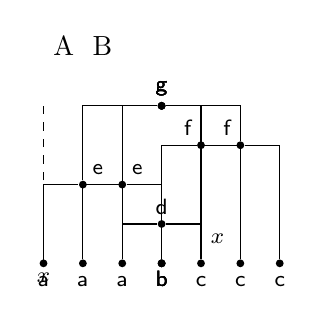
\begin{tikzpicture}[x=5mm, y=5mm, node distance=2mm and 20mm]
\tikzset{greynode/.style={circle,fill,inner sep=1},
nodelabel/.style={font=\footnotesize}}


\node [anchor=north west] at (\x1,6) {A};
\node [anchor=north west] at (\x2,6) {B};
% \node [anchor=north west] at (\xt,6) {C};

%%% (A) ARG

\node (s0) [greynode] at (\x1 + 0, 0) {};
\node (s1) [greynode] at (\x1 + 3, 0) {};
\node (s2) [greynode] at (\x1 + 6, 0) {};
\node (s3) [greynode] at (\x1 + 3, 1) {};
\node (s4) [greynode] at (\x1 + 1, 2) {};
\node (s5) [greynode] at (\x1 + 5, 3) {};
\node (s6) [greynode] at (\x1 + 3, 4) {};

\draw (s1) -- (s3);
\draw (s0) |- (s4);
\draw (s4) -- (\x1 + 2,2) |- (s3);
\draw (s4) |- (s6);
\draw (s3) -- (\x1 + 4,1) |- (s5);
\draw (s2) |- (s5);
\draw (s5) |- (s6);

%%% (B) Trees
\node (l0) [greynode] at (\x2 + 0, 0) {};
\node (l1) [greynode] at (\x2 + 2, 0) {};
\node (l2) [greynode] at (\x2 + 3, 0) {};
\node (l3) [greynode] at (\x2 + 1, 2) {};
\node (l4) [greynode] at (\x2 + 2, 4) {};

\draw (l0) |- (l3);
\draw (l1) |- (l3);
\draw (l2) |- (l4);
\draw (l3) |- (l4);

\node (r0) [greynode] at (\x3 + 0, 0) {};
\node (r1) [greynode] at (\x3 + 1, 0) {};
\node (r2) [greynode] at (\x3 + 3, 0) {};
\node (r3) [greynode] at (\x3 + 2, 3) {};
\node (r4) [greynode] at (\x3 + 1, 4) {};

\draw (r0) |- (r4);
\draw (r1) |- (r3);
\draw (r2) |- (r3);
\draw (r3) |- (r4);

\foreach \u/\lab in {
        s0/$\noderef{a}$, s1/$\noderef{b}$, s2/$\noderef{c}$,
        r0/$\noderef{a}$, r1/$\noderef{b}$, r2/$\noderef{c}$,
        l0/$\noderef{a}$, l1/$\noderef{b}$, l2/$\noderef{c}$}
    \node[nodelabel,anchor=south] at ([yshift=-12pt]\u) {\lab};

\foreach \u/\lab in {
        s6/$\noderef{g}$,
        l4/$\noderef{g}$,
        r4/$\noderef{g}$}
    \node[nodelabel,anchor=south] at (\u) {\lab};

\node [nodelabel,anchor=north west] at ($(s3) + (\x1 + 0,0)$) {$x$};
\foreach \u/\lab in {
        s4/$\noderef{e}$,
        l3/$\noderef{e}$}
    \node[nodelabel,anchor=south west] at (\u) {\lab};
\foreach \u/\lab in {
        s5/$\noderef{f}$,
        r3/$\noderef{f}$}
    \node[nodelabel,anchor=south east] at (\u) {\lab};
\foreach \u/\lab in {s3/$\noderef{d}$, s6/$\noderef{g}$}
    \node[nodelabel,anchor=south] at (\u) {\lab};

\draw[dashed] (\xx,0) -- (\xx, 4);
\node[nodelabel,anchor=north] at (\xx,0) {$x$};


% %%% (C) Encoding
% \node [nodelabel,anchor=north west] at ($(\xt,5)$) {
% \begin{tabular}{c|c|l}
% % \multicolumn{2}{c}{Breakpoints}\\
% Node & Breakpoint & Parents\\
% \hline
% $\noderef{a}$ & $\varnothing$ & [\noderef{e}]\\
% $\noderef{b}$ & $\varnothing$ & [\noderef{d}] \\
% $\noderef{c}$ & $\varnothing$ & [\noderef{f}]\\
% $\noderef{d}$ & $x$ & [\noderef{e}, \noderef{f}] \\
% $\noderef{e}$ & $\varnothing$ & [\noderef{g}]\\
% $\noderef{f}$ & $\varnothing$ & [\noderef{g}]\\
% $\noderef{g}$ & $\varnothing$ & []\\
% \end{tabular}};

\end{tikzpicture}
\caption{\label{fig-event-arg}
A classical event ARG (eARG). (A) Standard graph depiction with
breakpoint $x$ associated with the recombination node \noderef{d}.
Nodes \noderef{e}, \noderef{f} and \noderef{g} are common ancestor events.
(B) Corresponding local trees to the left and right of breakpoint $x$
(note these are shown in the conventional form in which only coalescences
within the local tree are included; see Section~\ref{sec-ARG-and-local-trees}
for a discussion of this important point).
}
\end{figure}

% eARGs are representationally for limited interchange
While the Griffiths approach of annotating recombination nodes with a
breakpoint in an eARG is a concise and elegant way of describing realisations
of the coalescent, it is inherently limited when
implemented literally. The eARG encoding explicitly models only
two different types of event and thus anything that is not a single crossover
recombination or common ancestor event, must be incorporated
either in a roundabout way using these
events, or by adding new types of event to the encoding. For example, gene
conversion could be accommodated either by stipulating a third type of event
(annotated by two breakpoints and corresponding traversal conventions for
recovering the local trees) or by two recombination nodes joined by a
zero-length edge. From the perspective of practical interchange of data between
inference methods and downstream applications, both
workarounds are problematic, and the gARG encoding described in the previous
section offers a much simpler solution.

Aside from these obvious practical challenges arising from a
literal implementation of the Griffiths approach, there is a deeper
issue with the implicit strategy of basing an ARG data structure on
recording events and their properties (e.g.\ the crossover breakpoint
for a recombination event). The fundamental problem
is that this approach assumes all events are \emph{knowable}, and does not
provide any obvious mechanism for either aggregating multiple events
or expressing uncertainty about them. While this is not a
problem when describing the results of simulations (where all details
are perfectly known), it is a major issue when we wish to
formally describe the output of inference methods, particularly
as datasets approach the population scale.
As discussed in the introduction,
the precise details of all events in these vast ARGs can never be
known, and a data structure that \emph{enforces} complete
precision is therefore an impediment to progress.

There is also a certain clarity gained by explicitly modelling nodes
in the inheritance graph as genomes.
Outside of the context of a
% The point being, events are perfectly well defined in the models
% but not in reality
mathematical model, an ``event'' is a slippery concept.
For example, \emph{which} genome along a chain of cell divisions should be
regarded as the one where an event occurred,
or whether multiple coalescences
within a single individual should be regarded as one or multiple events are
debatable points (Appendix~\ref{sec-cell-lineages-and-args}).
% If we want to have an ARG software ecosystem then such fireside
% discussions won't help.
From the perspective of a concrete data structure,
ideally forming the basis of an ecosystem of interoperable
inference and analysis methods, such debates
are unproductive.

\section{Ancestral material and sample resolution}
\label{sec-ancestral-material}
Ancestral material~\citep{wiuf1999ancestry,wiuf1999recombination}
is a key concept in understanding the overall inheritance structure
of an ARG (here, and throughout, we use the general term ``ARG'' when
the details of the specific encoding are not important).
It denotes the genomic intervals ancestral to a set of samples
on the edges of an ARG.
For example, in Fig.~\ref{fig-arg-in-pedigree} we have
four sample genomes, \noderef{a}--\noderef{d}. As we
trace their genetic ancestry into the previous generation
(\noderef{e}--\noderef{h}), we can think of their ancestral
material propagating through the graph
backwards in time. In the region $[2, 7)$, there is a
local coalescence where nodes \noderef{a} and \noderef{c}
find a common ancestor in \noderef{f}. Thus, in this region,
the total number of genome segments that are ancestral to the
sample is reduced from four to three. Fig.~\ref{fig-arg-in-pedigree}A
illustrates this by (shaded) ancestral material being present
in only three nodes (\noderef{f}, \noderef{g}, and \noderef{h}) in this region,
while node \noderef{e} is blank
as it carries \emph{non-ancestral} material.
This process of local coalescence continues through the
graph, until all samples reach their most recent common
ancestor in node \noderef{n}.

The process of tracking local coalescences and updating
segments of ancestral material is a core element of
Hudson's seminal simulation
algorithm~\citep{hudson1983testing,kelleher2016efficient},
and the key distinguishing feature between the
``Big'' and ``Little'' ARG stochastic processes
(see Appendix~\ref{sec-big-and-little-arg}).
The ability to \emph{store} resolved ancestral material
is also a key distinction between the eARG and gARG
encodings. Because an eARG stores only the graph topology and
recombination breakpoints, there is no way to locally
ascertain ancestral material without traversing the graph
pastwards from the sample nodes,
resolving the effects of recombination and common ancestor events.

Efficiently propagating and resolving ancestral material for
a sample through a pre-existing graph is a well-studied problem,
and central to recent advances in individual-based forward-time
simulations~\citep{kelleher2018efficient,haller2018tree}.
In contrast to the usual ``retrospective'' view of ARGs
discussed so far, these methods record an ARG forwards in
time in a ``prospective'' manner. Genetic inheritance relationships
and mutations are recorded exhaustively, generation-by-generation,
leading to a rapid build-up of information, much of which
will not be relevant to the genetic ancestry of the current population.
This redundancy is periodically removed using the ``simplify''
algorithm~\citep{kelleher2018efficient}, which propagates and
resolves ancestral material.
Efficient simplification is the key enabling factor for
this prospective-ARG based approach to forward-time simulation,
which can be orders of magnitude faster than standard
sequence-based methods
(see Section~\ref{sec-ARG-simplification} for
other applications of ARG simplification).
% Define "sample-resolved" here for later use
We refer to a gARG that has been simplified with respect to a set of
samples, such that the inheritance annotations on its edges contain
no non-ancestral material,  as sample-resolved.

\begin{figure}
\centering
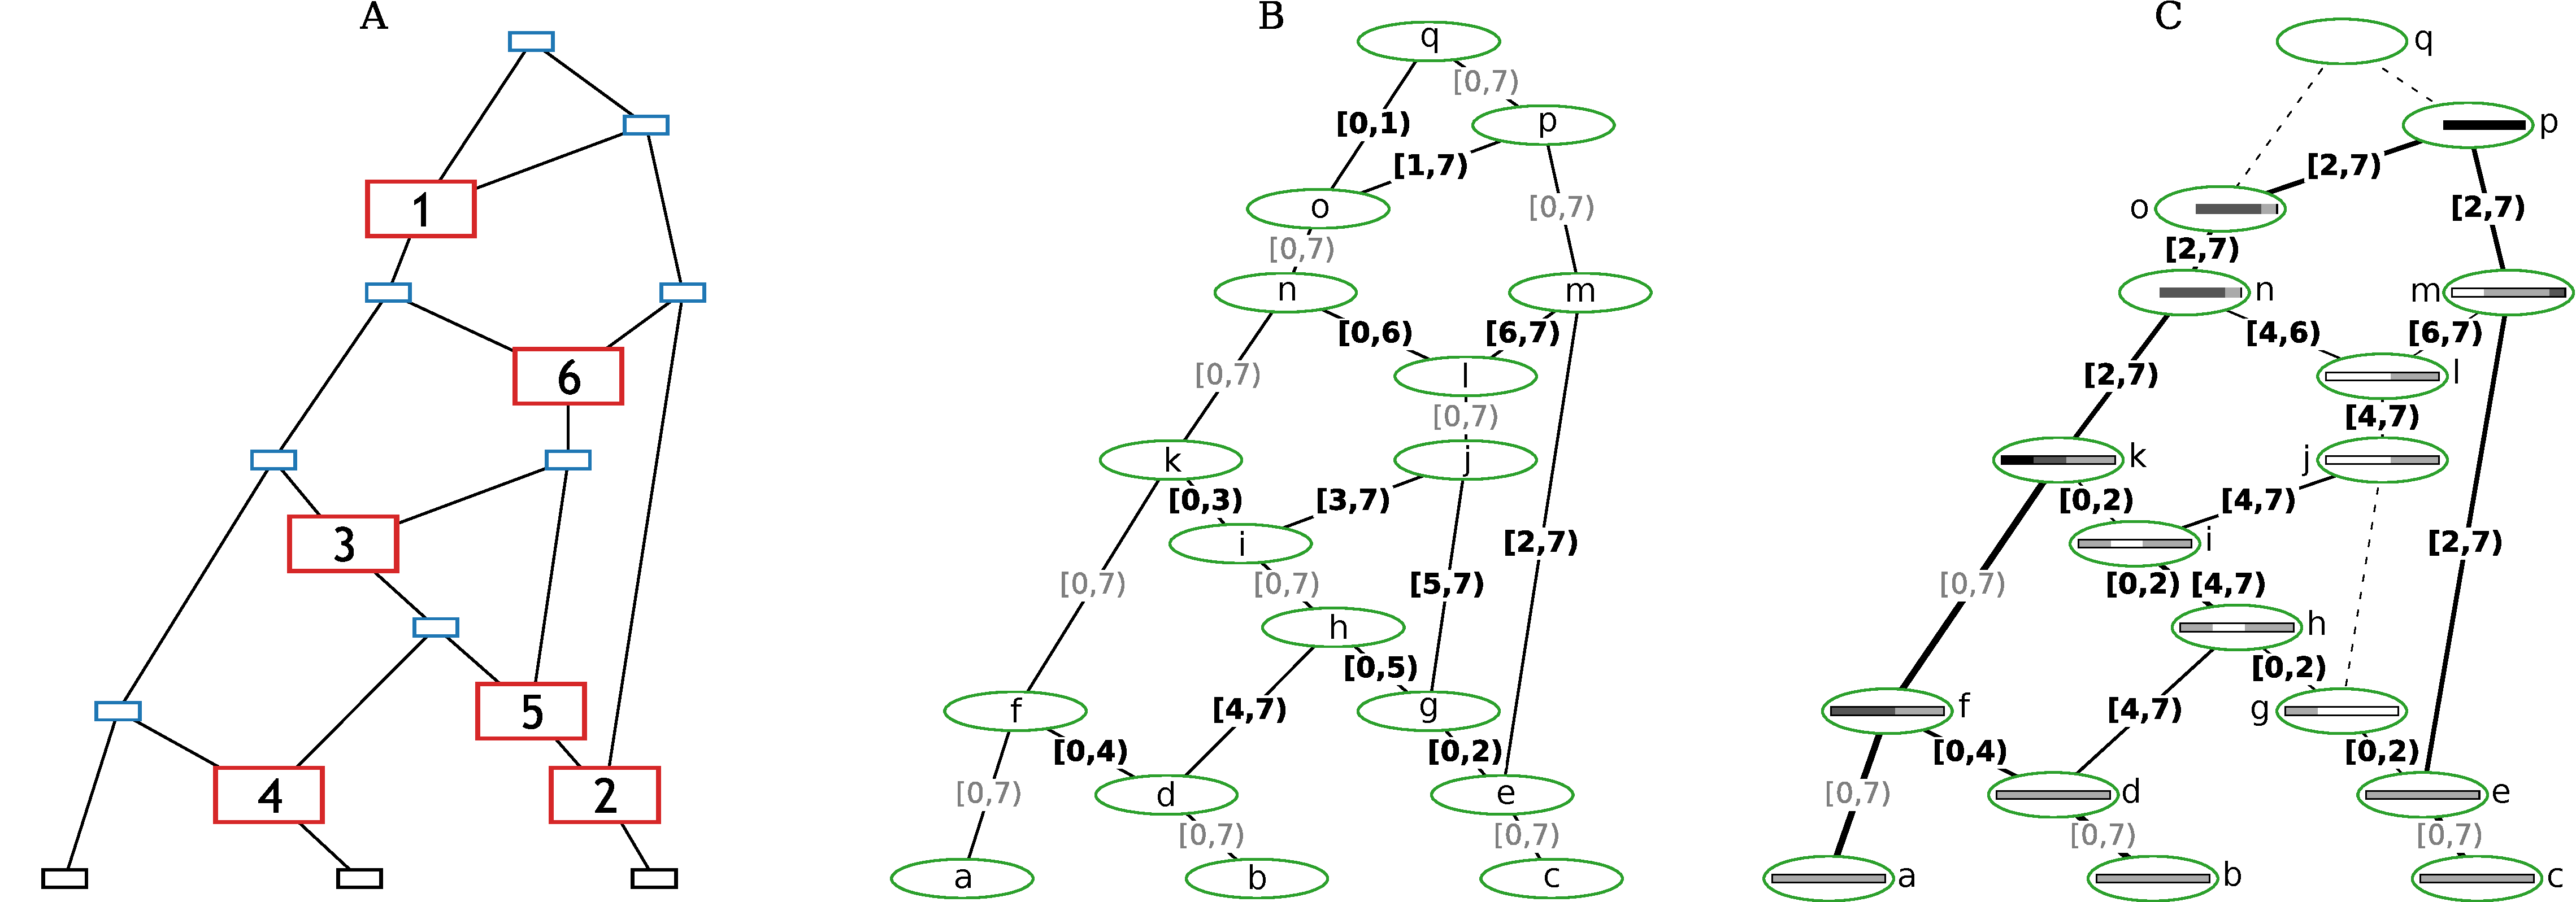
\includegraphics[width=\textwidth]{illustrations/ancestry-resolution}
\caption{\label{fig-ancestry-resolution}
Converting the \citet[][Fig.~1]{wiuf1999recombination} example
to a sample-resolved gARG. (A) The original eARG; square nodes
represent sampling (black), common ancestor (blue), and recombination (red) events;
the latter contain breakpoint positions.
(B) The corresponding gARG with breakpoints directly converted to
edges annotated with inheritance intervals.
(C) The sample-resolved gARG resulting from simplifying with respect
to the sample genomes, \noderef{a}, \noderef{b}, and \noderef{c}.
Dashed lines show edges that are
no longer present (in practice, nodes \noderef{g}, \noderef{j}, and \noderef{q} would also be removed).
Coalescence with respect to the sample is indicated by shaded bars, as
in Fig.~\ref{fig-arg-in-pedigree}A; nodes \noderef{n}, \noderef{o}, \noderef{p}, \noderef{q} have truncated
bars showing that local ancestry of entirely coalesced regions is omitted.
Line thickness is proportional to the genomic span of each edge.
Nodes representing recombination events are retained
for clarity, but could be removed by simplification if
desired.
}
\end{figure}

Any eARG can be converted to a sample-resolved gARG
via a two-step process illustrated in Fig.~\ref{fig-ancestry-resolution}.
The first step is to take the input eARG (Fig.~\ref{fig-ancestry-resolution}A),
duplicate its graph topology, and then add inheritance annotations
to each of the gARG's edges (Fig.~\ref{fig-ancestry-resolution}B) as follows.
If a given node is a common ancestor event, we annotate the single
outbound edge with the interval $[0,L)$, for a genome of length $L$. If the
node is a recombination event with a breakpoint $x$, we annotate the two
outbound edges respectively with the intervals $[0, x)$ and $[x, L)$. These
inheritance interval annotations are clearly in one-to-one correspondence with
the information in the input eARG. They are also analogous to the
inheritance intervals we get on the edges in a prospective gARG
produced by a forward-time simulation, which are concerned with recording
the direct genetic relationship between a parent and child genome and are not
necessarily minimal in terms of the resolved ancestral material of a sample.
Thus, the final step is to use the ``simplify'' algorithm to perform the required
sample resolution (Fig.~\ref{fig-ancestry-resolution}C).

The sample-resolved gARG of Fig.~\ref{fig-ancestry-resolution}C
differs in some important ways to the
original eARG (Fig.~\ref{fig-ancestry-resolution}A).
Firstly, we can see that some nodes and edges have been removed entirely
from the graph.
The ``grand MRCA'' \noderef{q} is omitted from the
sample-resolved gARG because all segments of the genome have
fully coalesced in \noderef{k} and \noderef{p} before \noderef{q} is reached.
Likewise, the edge
between \noderef{g} and \noderef{j} is omitted because the recombination
event at position $5$ (represented by node \noderef{g})
fell in non-ancestral material.
More generally, we can see that the sample resolved
gARG of Fig.~\ref{fig-ancestry-resolution}C
allows for ``local'' inspection
of an ARG in a way that is not possible in an eARG.
Because the ancestral material is stored with each edge of a gARG, the
cumulative effects of events over time can be reasoned
about, without first ``replaying'' those events.
Many computations
that we wish to perform on an ARG will require resolving
the ancestral material with respect to a sample.
% this is weak, but would be good to emphasise this point.
% you just end up running simplify lots of times, in your
% downstream algs
The gARG encoding
allows us to perform this once
and to store the result,
whereas the eARG encoding requires us to repeat the process
each time.

Note that the \citet{wiuf1999recombination} eARG
in Fig.~\ref{fig-ancestry-resolution} is not particularly
representative, because inference or simulation methods usually
only generate ARGs containing nodes and edges ancestral to the sample
(but see the discussion of the ``Big ARG'' stochastic process in
Appendix~\ref{sec-big-and-little-arg}).
Nonetheless, it is an instructive example from the literature which highlights several
important properties of ARGs, and the general point about
the need to resolve ancestral material ``on the fly'' for eARG traversals
holds.

\section{ARGs and local trees}
\label{sec-ARG-and-local-trees}
% (We use ``local'' rather than
% ``marginal''
% % could list loads here, but not much point.
% trees~\citep[e.g.][]{griffiths1996ancestral,minichiello2006mapping,kelleher2016efficient}
% to avoid the potential confusion with the
% statistical concept of marginal distributions.)
The relationship between an ARG and its corresponding
local trees is subtle and important.
A fundamental property of genetics is that a
given DNA nucleotide is inherited from exactly one parent genome,
both at an organismal and cell-by-cell level
(Appendix~\ref{sec-cell-lineages-and-args}).
These paths of single-parent inheritance give rise,
by definition, to a tree structure.
As a result of recombination, adjacent nucleotides can have
different paths of inheritance, and
an ARG encodes the entire ensemble of local trees along the
% Said "sample of genomes" originally, but using term "genome" in two
% different ways in the same sentence then.
genome for a given set of sample nodes.
% This is for Yan - to me this is a given, but maybe some people feel
% the following is overly formal?
Precisely defining the process by which local trees are extracted
from an ARG is essential to our understanding of how ARGs and local trees
are related, and we require a concrete mathematical structure
to describe the local trees. It is important to note that
although the following discussion is phrased in terms of the
gARG encoding,  the arguments apply equally to eARGs
because any eARG can be converted to a
% Note, being sample-resolve is not necessary for following argument so omitting
gARG without loss of information (Section~\ref{sec-ancestral-material}).

Oriented trees provide a
convenient formalism to capture these parent-child relationships
in a well-defined combinatorial object.
% There's no need for a comma
Let $\pi_1\dots\pi_n$ be a sequence of integers, such that $\pi_u$
denotes the parent of node $u$, and $\pi_u = 0$ if $u$ is a
root~\cite[p.\ 461]{knuth11combinatorial}.
This encoding is particularly useful to describe
evolutionary trees because parent-child relationships are
important but the ordering of children at a node is
not~\citep{kelleher2013coalescent,kelleher2014coalescent,
kelleher2016efficient}.
Thus, for a given gARG with nodes $\{1, \dots, n\}$ and
edges $E$ (Section~\ref{sec-gARG}), we recover the local tree
at position $x$ as follows.
We begin by setting $\pi_u = 0$ for each $1 \leq u \leq n$.
Then, for each sample node in $S$ we trace its path pastwards through the
ARG for position $x$, and record this path in $\pi$.
Specifically, at a given node $u$,
we find an edge $(c, p, I) \in E$ such that $u = c$ and $x \in I$, and set
$\pi_c \leftarrow p$. We then set $u \leftarrow p$, and repeat
until either $\pi_u \neq 0$ (indicating we have traversed this section
of the ARG already on the path from another sample) or there
is no matching outbound edge (indicating we are at a root).
Note that the local trees for an ARG are ``sparse''~\citep{kelleher2016efficient},
because many ancestral nodes will not be reachable from the
samples at a given position (so their corresponding entries in $\pi$ will be zero).

This combinatorial approach provides at least
one novel insight, clarifying the fundamental relationship between
ARGs and local trees.
Suppose we are given a gARG defined by a set of nodes and edges.
There is no requirement on the structure of this ARG beyond
the basic definitions: it could correspond to an ARG in which
every recombination event is exactly specified
(e.g.\ Fig.~\ref{fig-ancestry-resolution})
or one in which local trees are entirely disjoint
(i.e.\ only the sample nodes are shared between them).
If we  are given the sequence of local trees for this gARG
encoded as an oriented tree, along with the genome interval
covered by each tree, we can recover the original gARG exactly.
% We do this site-by-site for simplicity, but hopefully it's obvious
% that this isn't necessary?
More formally, suppose we are given the local tree $\pi^x_1\dots\pi^x_n$
for each nucleotide position $1 \leq x \leq L$ on a genome of length $L$.
Then, the edges of the ``local ARG'' for this tree is given by
$E^x = \{(u, \pi_u^x, \{x\}) \mid \pi_u^x \neq 0\}$. Because the ARG
edges are defined by $(c, p, I)$ tuples, where the set $I$ defines
the positions over which node $c$ inherits from parent $p$, we can
then simply combine the ``local ARGs'' for each position $x$
% YW: The above "combining" operation isn't obviously lossless to me:
% we could potentially lose information in the different combinations
% of intervals (e.g. if we use 2 non-combined intervals to represent a
% diamond in a 1-RE-node ARG). It seems like we might need an additional
% gARG spec to define what combinations of intervals are equivalent.
% But no-one else has commented on this, so I guess we just let it lie.
to recover precisely the same set of edges as the original ARG.
Thus, under this definition, there
is a one-to-one correspondence between an ARG and
the sequence of local trees that it encodes.

This is not the prevailing view, however.
\cite{kuhner2017consensus} argue that the
``interval-tree'' representation of
an ARG (the local trees and the genome intervals they cover)
``does not contain all of the information in the underlying ARG: it lacks the
number of recombinations occurring at each site, the times at which
recombinations occurred, and the specific sequences involved as recombination
partners.''
\cite{shipilina2023origin} discuss the same ideas,
and note that the
``full ARG...~contains more information than the series of tree
sequences along the genome''.
These
% % Could cite some more? E.g. KwARG paper says
% % "We note that ARGs contain more information than local trees"
% % Would need a few more examples though, which would require some digging.
%
% and similar, \citep[e.g.][]{}
statements that an ARG
contains more information than its local trees are true
if we represent local trees in their conventional forms,
but these forms discard important information that is
available in an ARG.

There are two properties of how evolutionary trees are conventionally
represented that lead to this
disagreement about the relationship between local trees and an ARG.
Firstly, the internal nodes of evolutionary trees are usually considered to be
\emph{unlabelled}, or equivalently, labelled by the leaves which they subtend.
The same canonical labelling cannot be used for internal ARG nodes because the
leaves they subtend will typically vary by genomic position. If we do not label
the tree nodes in a way which is persistent across the sequence of local trees
in the ARG, we lose the fact that the \emph{same} ancestors sometimes persist
across multiple trees.
Defining ARG nodes as integers and using the oriented
tree encoding explicitly labels internal nodes, and makes the relationship
between tree and ARG nodes clear and precise.

% Note: good to keep to paras here to logically separate the two important
% points.
The second property of how evolutionary trees
are conventionally represented that is unhelpful in the context of ARGs is their
focus on branching points (coalescences), i.e.\ nodes that have two or more children.
As the introductory paragraph of this section emphasised,
parent-child relationships are what fundamentally define a tree,
and branching points can be seen as incidental. This is reflected
by the oriented tree encoding which simply stores the local
parent-child relationships, and does not, for example,
directly tell us how many children a particular node has.
The local tree at a given position records the \emph{path} through
the ARG; if this path omits nodes that are not
branching points (such as \noderef{e} in Fig.~\ref{fig-arg-in-pedigree}),
we lose information about the ARG.
We return to this point in the following two sections,
when we discuss ``locally unary'' nodes and the simplification process.

It is important that we make the distinction here between the local
trees that we can derive from a known ARG (as just discussed),
and an ARG that we can derive from a sequence of \emph{estimated}
local trees.
The ARG inference method
\espalier~\citep{rasmussen2022espalier} is illustrative in this context.
It begins by splitting an input sequence alignment into
segments that are assumed to be non-recombining. Within
each segment, an initial local tree is estimated using
standard phylogenetic methods. By necessity, these local
trees will contain internal nodes that are unlabelled and
consist only of branching points: there is no information
shared between the independent tree estimation steps
across segments. Part of the task of stitching
these trees together
into an ARG is then, essentially, to generate labels for
the internal nodes, and decide which nodes persist
across multiple local trees.
\espalier\ approaches this task
by identifying maximal subtrees
that do not change between pairs of adjacent
local trees and then
heuristically exploring the space of possible
rearrangements of these subtrees.
To derive details about recombination events,
\espalier\ then attempts to infer
the precise subtree prune-and-regraft (SPR)
operations~\citep{hein1990reconstructing,song2003on,song2006properties}
induced by recombination between these partially reconciled local trees.
% NOTE: dropping this because it doesn't clarify the actual point.
% A similar problem is tackled by \arbores~\citep{heine2018bridging}, which
% explores a space of ARGs by fixing a starting ARG, and then repeatedly erasing
% and resimulating candidate SPR moves connecting two fixed, leaf-labelled local
% trees.
Inferring the SPRs between leaf-labelled trees is
NP-hard~\citep{hein1996complexity,allen2001subtree,bordewich2005computational},
but it is unclear what the complexity is when there
is a degree of internal node sharing between trees.
% I don't really know if this is true, it's just a way of wrapping the
% section up by saying that other things we thought were settled might
% be worth thinking about again.
The combinatorial formulation of ARGs and local trees provided here
may help clarify these fundamental questions.

\section{Locally unary nodes}
\label{sec-locally-unary-edges}
As discussed in the previous section, the local tree at a given position
$x$ is best seen as the path through the ARG at that position, defined
by the oriented tree $\pi^x_1\dots\pi^x_n$. This path does not directly
contain information about branching points, and defining a
node's arity (number of child nodes) is therefore useful.
The ``local arity'' of a node is the number of children it has
in the local tree at position $x$, i.e., $a^x_u = |\{v : \pi^x_v = u\}|$
for each $1 \leq u \leq n$. The ``ARG arity'' of a node $u$ is the
number of children it has in the graph topology, i.e.\
$a_u = |\{v: (v, u, I) \in E\}|$. Thus, the local arity is less than
or equal to the ARG arity (more precisely, $0 \leq a^x_u \leq a_u$),
and the local arity of a node may change as we move along the genome.

This distinction between ARG and local arity is mainly
of interest when we consider nodes that have
a single child: those that are \emph{unary}.
Returning to the example in Fig.~\ref{fig-arg-in-pedigree}, nodes
\noderef{g} and \noderef{h}
are ARG-unary (Fig.~\ref{fig-arg-in-pedigree}B), and are consequently
also unary in the local trees (Fig.~\ref{fig-arg-in-pedigree}C).
On the other hand, node \noderef{f} has two children
in the graph, but is binary only
in the local tree covering the interval $[2, 7)$,
representing the coalescence of samples \noderef{a} and \noderef{c}
in this genome region. Over the interval $[0, 2)$ no coalescence occurs,
but we still record the fact that genome \noderef{c} inherits from \noderef{f}
in the local tree. Thus, node \noderef{f} has a single child in this
interval: it is \emph{locally unary}.
In another example, \noderef{e} is binary in the graph, being a common
ancestor of \noderef{a} and \noderef{c}, but is
locally unary in all trees in which it is present.
This is because no ancestral material coalesces in \noderef{e}:
\noderef{a} inherits genetic material from the far left hand end of
\noderef{e},
while \noderef{c} only inherits the (disjoint) right hand end.

% We get discussion of ARG-unary nodes out of the way first: these are
% relatively easy to understand (but it's worth emphasising that
% eARG-like recombination nodes are ARG-unary, as that might not be clear
By definition, ARG-unary nodes have one child but can have one or
more parents.
A node with one child and only one parent represents a ``pass-through'' node:
these occur where we wish the record the passage of ancestral material
through a known node. For example, in simulations
it is sometimes useful to record the passage of
ancestral material through known pedigree individuals
regardless of whether common ancestry occurs.
Nodes with one child and two parents arise when
we model a recombination event using a single node
in the classical manner
(e.g.\ Fig.~\ref{fig-ancestry-resolution}).
It is also possible for sample nodes to be ARG-unary, for example
in inferences from longitudinal datasets where genetic
data is sampled at many timepoints and recombination
is rare (e.g.~SARS-CoV-2; see Discussion).

% Moving on from ARG-unary to the more general case
More generally, locally unary nodes,
which can have one or more children in the graph,
are a common and important feature
of many different types of ARG.
As discussed in the previous section,
without these nodes marking the passage
of ancestral material through specific ancestors, the local trees
lack information about events other than local coalescence.
% Not sure if switching example will confuse people here, but would
% like to contrast with example where we don't use unary nodes to
% emphasise the point that we lose info
For example, the local trees for the classical event ARG
depicted in Fig.~\ref{fig-event-arg}B follow the usual conventions
and do not include any information about the recombination
that occurred at node \noderef{d}. Given these two local trees
in isolation
% (without further information about the corresponding ARG)
we lack specific information about the recombination.
Explicitly recording that node \noderef{d} lies on the
branch joining \noderef{b} to \noderef{e} in the left hand
tree, and \noderef{b} to \noderef{f} in the right hand tree
resolves all ambiguity, and makes the collection of local
trees exactly equivalent to the corresponding ARG (see previous section).
Unary nodes are a vital link between ARGs and local trees, and we
cannot fully reason about how a local tree is embedded in an ARG
without them. As we see in the next two sections, both ARG and locally
unary nodes occur in various scenarios, and are
produced by a range of current inference methods.

\section{Levels of simplification}
\label{sec-ARG-simplification}
ARG simplification is a powerful tool.
In general, we can think of
simplification as the process
of removing nodes and re-writing edges (and their inheritance annotations)
to remove various types of redundancy, much of which
% We are interested in both graph and local unary, so qualifying this
% would just make it less readable, IMO
revolves around the presence of unary nodes (see previous section).
We illustrate this successive removal of redundancy
through a series of simplification steps
in Fig.~\ref{fig-simplification}.

\begin{figure}
\centering
\includegraphics[width=\textwidth]{illustrations/simplification}
\caption{\label{fig-simplification}
Levels of ARG simplification.
(A) An example gARG simulated from a diploid Wright-Fisher model.
(B) Remove all
singly-connected graph components (e.g., diamonds such as \noderef{jlnm}).
(C) Remove nodes that never represent coalescences,
i.e.\ are unary everywhere (e.g.\ \noderef{n} and \noderef{r}).
(D) Rewrite edges to bypass nodes in local trees in which they are unary.
In each case, the graph is shown on the left
and corresponding local trees on the right.
% Repetition here, but I'm thinking about the casual "I'm just reading
% the captions reader" who might not realise that there's an essential
% ingredient missing from the graph version
In the interest of visual clarity, inheritance intervals are not shown
on the graph edges; Supplementary Fig.~\ref{fig-simplification-with-edges}
shows the graphs with these inheritance intervals included.
Graph nodes are coloured by the number of parents and shaded
according to the proportion of their span over which they are coalescent;
see the text for more details.
}
\end{figure}

The ARG in Fig.~\ref{fig-simplification}A is the output of a
backwards-time Wright-Fisher simulation for a sample of two diploid
individuals (population size $N=10$), and follows a similar process
to the methods described by~\cite{nelson2020accounting}.
As we proceed backwards in time, generation by generation, the
extant lineages choose parents randomly.
With a certain probability recombination occurs, and the ancestral
material of a lineage is split between the two parental
genomes. Local coalescence occurs
when lineages with overlapping ancestral material choose the same
parent genome.
Note that in this simulation we do not explicitly
model recombination \emph{events} via an ARG node, but simply record
the \emph{outcome} of a recombination via edges to
the parent's two genomes.
Thus, a recombinant node such as \noderef{g} in Fig.~\ref{fig-simplification}
may also correspond to a coalescence.
The distinction of
using a single node to represent
a recombination event, as is done in ~Fig.~\ref{fig-ancestry-resolution},
or two to represent the parent genomes, as in Fig.~\ref{fig-simplification},  is usually not important.
Either is possible in the gARG encoding, and the most convenient approach will vary by application
(discussed e.g.\ in Appendix~\ref{sec-big-and-little-arg}).
Note also that node \noderef{k} in Fig.~\ref{fig-simplification} has three children.
Polytomies like this are a natural feature of such a Wright-Fisher model
(but see Appendix~\ref{sec-cell-lineages-and-args}).

The graph visualisations in Fig.~\ref{fig-simplification} have
three novel features which require some explanation.
Firstly, edge weights (the thickness of the lines joining
nodes) correspond to the length of the inheritance intervals
they are annotated with. This allows us to distinguish
edges that persist across many local trees from those that are
less influential (contrast the edge
$(\noderef{g}, \noderef{h})$
with $(\noderef{g}, \noderef{i})$
in Fig.~\ref{fig-simplification}A).
Secondly, node colours denote the number of parents that they
have in the graph, allowing us to easily see roots (those
with zero parents), recombinants (those with two parents)
and more complex situations arising from simplification (see below).
Thirdly, the shading intensity of a node denotes the ``coalescent span'', the
fraction of the node's span (the length of genome in which it
is reachable from the samples in the local trees)
over which it has more than one child. Nodes which
are never locally unary therefore have a coalescent span of 100\%,
whereas nodes in which ancestral material never coalesces have a
coalescent span of 0\%.

Returning to the main topic of this section,
Fig.~\ref{fig-simplification}A is the original simulation output, in
which we retain all nodes involved in recombination
or common ancestry events. This is the true history, and contains
a very high level of detail, some of which may be considered
redundant (or, from another perspective, unobservable).
In Fig.~\ref{fig-simplification}A the local trees (right)
contain many unary nodes, fewer as  we successively
simplify (Fig.~\ref{fig-simplification}B,C),
until we reach Fig.~\ref{fig-simplification}D, where there are none.

The first level of simplification that we can perform is based only
on the graph topology.
An example of graph topology that we may consider redundant
(or non-identifiable) is a
``diamond''~\citep{rasmussen2014genome}
in which the two parent nodes of a recombination immediately
join again into a common ancestor (e.g.~\noderef{j}, \noderef{l}, \noderef{m}
and \noderef{n} in Fig.~\ref{fig-simplification}A).
Unless we are specifically
interested in the recombination event or these ancestral genomes,
the diamond can be replaced by a single edge without loss of
information.
More generally, any subgraph that is singly-connected in both the leafward and
rootward direction (a ``super-diamond'') can be replaced by one edge.
This definition includes the case
of a node that has one inbound and one outbound edge, such as
nodes \noderef{f} and \noderef{h}.
% Note that f and h are only removable because we are using the 2-RE-node
% representation. That means when we remove these nodes, we lose information about
% the time of recombination, which we wouldn't do if we were using the
% 1-RE-node representation (because the node would be multiply connected
% in the rootward direction). We definitely don't want to get into this
% level of detail here though, so we'll just pass over it without comment.
Fig.~\ref{fig-simplification}B shows the result of this type of
graph topology simplification.

Simplifying away diamonds will remove many unary nodes from the
local trees, but there can still be nodes that are unary in all
of the local trees. In particular, a node can represent a recombinant
with multiple parents in the graph but only a single child (e.g.\ node \noderef{n}
in Fig.~\ref{fig-simplification}B), or can represent a common ancestor with
multiple children in the graph but in which no coalescence takes place
in the local trees
(node \noderef{r} in Fig.~\ref{fig-simplification}B).
The distinction between the ``common ancestry'' of two or more genomes
in an ancestral genome and the ``coalescence'' which may or may
not occur in the local trees is
important~\citep{hudson1983testing,kelleher2016efficient}.
Consider \noderef{e} in Fig.~\ref{fig-simplification}A,
for example. We can see from the graph that it is a common
ancestor of samples \noderef{a} and \noderef{b}, but
it does not correspond to any coalescence in the
local trees to the left of position $44$, and is therefore
unary in these three trees.
Such nodes are not singly connected in the graph, but are nevertheless unary in
all of the local trees.
The operation to remove them
therefore requires knowledge not just of the graph topology but also of the
ancestral material associated with the edges.
As we see in Fig.~\ref{fig-simplification}C,
removal of recombinant nodes can produce graph nodes with
more than two parents (e.g.~node \noderef{e}); and likewise, removal of
common ancestor but non-coalescent nodes can produce graph nodes with
more than two children (e.g.~node \noderef{s}). Both cases represent the
merged
\emph{effects} of multiple evolutionary events in a single node (genome), and the
ARG no longer contains the intermediate genomes corresponding to
those events (see also Appendix~\ref{sec-cell-lineages-and-args}).

The remaining nodes are MRCAs of some subset of the samples
at \emph{some} positions along the genome. We still have
some unary nodes in the local trees, but these nodes will
correspond to a coalescence in at least one other
local tree. For example, node  \noderef{k} is unary in the fourth tree
of Fig.~\ref{fig-simplification}C, but is either binary
or ternary in all other local trees (recall this is a Wright-Fisher
simulation). The final level of simplification is to alter the edge annotations
such that, although no nodes are removed from the graph, all
unary nodes disappear from the local trees (Fig.~\ref{fig-simplification}D).
Note that although this last stage produces simpler local trees, by
removing information about the exact paths taken by lineages through
the graph, we lose potentially useful information about shared edges
between trees.
The \texttt{msprime} simulator, and the version of Hudson's algorithm described
by~\citet{kelleher2016efficient}, produces ARGs
that are fully simplified (i.e., contain no locally unary nodes).
It is not difficult, however, to update
these methods to record information about the passage of ancestral
material through genomes under a range of conditions.

An important consequence of simplifying ARGs to remove
unary nodes in local trees is that we lose some information
about recombination
events. This is related to the amount of \emph{precision} about
recombination events that we store and
can hope to infer from sampled genomes, which is the topic of the next
section.

\section{Precision of recombination information}
\label{sec-precision}
% The ARGs in Fig.~\ref{fig-simplification} represent different
% levels of detail about the same ancestral history. They represent
% the same set of recombination and common ancestor events,
As illustrated in Fig.~\ref{fig-simplification}, successive levels
of ARG simplification reduce the amount of information about the
history of the sample that is stored. Some of the information lost,
e.g.\ ``diamond'' removal (Fig.~\ref{fig-simplification}A),
seems like a reasonable tradeoff for a simpler structure.
The consequences of other simplifications, however, are
more subtle and relate directly to what can be known about
recombination events and the levels of precision that
we should seek to infer about them.

The ARGs in Fig.~\ref{fig-simplification} contain different
numbers of local trees ($6$, $5$, $5$ and $4$ respectively for A through
D). When we move from A to B the local trees
for the intervals $[44,61)$ and $[61,87)$ are merged because
the only differences between them are their paths through
nodes \noderef{l} and \noderef{m}. These nodes that participated
in the diamond are removed from the ARG, and we have lost
all information about the corresponding recombination at
position 61. Other nodes (e.g.\ \noderef{o} and \noderef{p})
have also been removed but these represent the \emph{parents}
of recombinants. The recombinant nodes themselves
(e.g. \noderef{n}) are still present, and represent precise
information about the time, genomic location and
lineages involved in the recombination event.

Fig.~\ref{fig-simplification}C has the same number of local trees
as Fig.~\ref{fig-simplification}B, but has less precise information
about recombination. Continuing the previous example, node
\noderef{n} has been removed from the graph because it was unary
in all of the local trees; its outbound edges to \noderef{s}
and \noderef{q} have effectively been ``pushed down''
to \noderef{e} (which is retained because it is the coalescent
parent of \noderef{a} and \noderef{b} over the interval
$[44, 100)$). We
have therefore lost precision about
the \emph{timing} of this recombination event, and know only
that it must have occurred between the times of node \noderef{e}
and \noderef{q}.

Fig.~\ref{fig-simplification}D removes all unary nodes from the
local trees, and further reduces the precision of
recombination information. Node \noderef{e} has not been
removed from the graph because it is coalescent in the
final tree, but we no longer know that the recombination
event at position 30 was ancestral to it, or have
any indication of its timings. Furthermore,
trees for $[44, 87)$ and $[87, 100)$ were only distinguishable
by the passage of the former tree through nodes \noderef{e}
and \noderef{q}, and so the recombination on node \noderef{g}
at position 87 has been lost entirely.

\section{Example inferred ARGs}
\label{sec-example-inferred-args}
The scalability gains made by recent ARG inference methods
such as \relate~\citep{speidel2019method} and
\tsinfer~\citep{kelleher2019inferring}
have been, in part, due to inferring lower levels of precision about
recombination than classical methods.
Neither method infers
explicit recombination events, and therefore their outputs cannot
be described using the classical eARG formalisms (Section~\ref{sec-eARG}).
% Could do, something like
% this mismatch has led some to characterise their output as a
% series of unrelated local trees [cite], which lacks nuance of the reality.
% Or maybe we don't bother: what's to be gained from pointing out people's
% mistakes here? Hopefully the rich detail of reality will come through
% and replace old ideas.
Nonetheless, both methods produce estimates in which nodes and edges
persist across multiple trees, creating
inheritance graphs which fit naturally into the gARG formulation.
To illustrate the varying levels of information captured
by current methods, and some qualitative differences between them,
Fig.~\ref{fig-inferred-args} shows graphical depictions of
example ARGs produced by four tools using substantially
different inference strategies.

\begin{figure} \begin{center}
\includegraphics[width=\textwidth]{illustrations/inference.pdf} \end{center}
\caption{\label{fig-inferred-args} Inference of sample-resolved ARGs for 11
\textit{Drosophila melanogaster} DNA sequences over a 2.4kb
region of the ADH locus~\citep{kreitman1983nucleotide}.
Results for four different methods:
(A) \kwarg; (B) \argweaver; (C) \tsinfer; and (D) \relate. See the
text for details of these methods.
Edge colours indicate time of the edge's child node
(lighter: older; darker: younger).
Vertical and horizontal positions of graph nodes are arbitrary.
Line width and node colour are as described in Fig.~\ref{fig-simplification}.
Bottom row graphics show the genome positions, relative to the start of
the ADH gene, for each graph edge from the corresponding ARG. Edge intervals
are drawn as horizontal lines, stacked in time order (edges with youngest
children at the bottom); vertical dashed lines denote breakpoints between
local trees.
}
\end{figure}

The first two methods explicitly infer recombination events.
\kwarg~\citep{ignatieva2021kwarg} is a parsimony based approach
which searches the space of plausible ARGs,
outputting minimal ones using heuristics.
\argweaver~\citep{rasmussen2014genome} on the other hand is
model-based, sampling from a discretised version of the
% could spell this out, but in reality everyone knows what the SMC
% is, and if they don't spelling it out won't help them.
SMC~\citep{mcvean2005approximating,marjoram2006fast}.
Note that both \kwarg\ and \argweaver\ produce many ARGs,
and those shown in Fig.~\ref{fig-inferred-args} are arbitrarily selected
examples.
While the second two methods
both produce a single best-guess estimate and
do not explicitly infer recombination events, they are based on
quite different principles.
\texttt{Tsinfer} works in a two-step process, first generating ancestral
haplotypes via heuristics and then inferring inheritance relationships
between them using the Li and Stephens model~\citep{li2003modeling}.
\texttt{Relate} first reconstructs local tree topologies across the genome,
using a variant of the Li and Stephens model to estimate the
ordering of coalescence events in each tree, and then estimates
branch lengths using MCMC with a coalescent-based prior.
See Appendix~\ref{sec-survey-arg-infer} for more details on these
and other inference methods.

Inferred ARGs are based on the \citet{kreitman1983nucleotide} dataset,
a standard benchmark in the classical ARG
literature.
It consists of 43 biallelic SNPs spanning 2.4Kb of the \emph{D.~melanogaster} ADH
locus on chromosome 2L. Where required for inference purposes we assume
mutation and recombination rates of $5.49\times10^{-9}$
and $2.40463\times10^{-9}$ per site per generation
\citep{schrider2013rates,comeron2012many}
and a constant effective population size of 1,720,600 \citep{li2006inferring},
as provided by the \texttt{stdpopsim}
catalog~\citep{adrion2020community,lauterbur2023expanding}.
Software versions were \kwarg~v1.0, \argweaverD~(2019),
\tsinfer~v0.3.1, and \relate~v1.1.9.
Full details and code for generating
these figures are available on GitHub (see Data Availability).

% Here we describe recombination features
Considering Fig.~\ref{fig-inferred-args}, we can see that
there is substantial variation in the number of recombination breakpoints
inferred by different methods, with e.g.~\argweaver\ suggesting
far more than the 7 required for this dataset under minimal parsimony
assumptions~\citep{song2003parsimonious}.
A sense of the amount of recombination in each ARG is provided by
the node colouring scheme, which shows the number of parents for each node.
In Fig.~\ref{fig-inferred-args}A,B, each recombination event
corresponds to a node with exactly two parents and one child.
As these methods explicitly infer a recombination event for each
breakpoint, the number of breakpoints equals the number of two-parent
(brown) nodes.
In contrast, Fig.~\ref{fig-inferred-args}C,D do not have this
straightforward
relationship between the number of nodes with multiple parents
and number of breakpoints along the genome.
In both ARGs the number of breakpoints is smaller
than the number of multiple-parent ARG nodes, showing
that several multiple-parent nodes must share breakpoint positions.
There are also ARG nodes with multiple parents and multiple children,
where one or more recombinations have been pushed down onto a
more recent node.
As a consequence, it may be difficult to condense each transition between trees
in these ARGs into a set of SPR operations.

% Here we move on to coalescence
Shading within nodes in Fig.~\ref{fig-inferred-args} indicates the
fraction of the node's span over which it is coalescent
(Section~\ref{sec-locally-unary-edges}). For example, brown nodes
in Fig.~\ref{fig-inferred-args}A,B are clear because there is
no local coalescence at these recombination nodes
(they are ``ARG unary'', and so local coalescence is impossible).
The significant number of partially shaded nodes in
Fig.~\ref{fig-inferred-args}A,B and C demonstrates that
the \kwarg, \argweaver\ and \tsinfer\ ARGs all contain locally unary nodes.
Another difference between methods highlighted in this figure
is the presence of polytomies, which only
\tsinfer\ creates. The most obvious example
involves nodes \noderef{Fr-F}, \noderef{Wa-F}, and \noderef{Af-F},
which happen to have identical sequences.
Because \kwarg, \argweaver, and \relate\ require
bifurcating trees by design, each picks an arbitrary order of branching
(hence Fig.~\ref{fig-inferred-args}A and B disagree
in this order, and Fig.~\ref{fig-inferred-args}D even shows different
orders in different trees).
% JK: I don't quite get the commented out sentence below, so readers probably
% won't either. Let's stick to a few clear messages.
% More generally, the number of nodes in Fig.~\ref{fig-inferred-args}C
% that have more than two children hints at considerable uncertainty in
% the order of branching elsewhere in the ARG.

The bottom row of Fig~\ref{fig-inferred-args} shows the extent along
the genome to which graph edges are shared between multiple trees.
All four methods infer nodes and edges that are shared between
multiple trees, to varying degrees.
For example, all of the methods infer
infer that \noderef{Af-f}, \noderef{Fr-f}, and \noderef{Wa-f}
form a clade along the entire sequence.
In particular, we can
see both \tsinfer\ and (to a lesser extent) \relate\ have edges
that span multiple tree boundaries, indicating that they are not inferring
a series of \emph{unrelated} local trees.
However, in comparison to \kwarg\ and \argweaver\ neither
method results in extensive node sharing in the
oldest time periods.
Overall, Fig.~\ref{fig-inferred-args} shows
that \tsinfer\ and \relate\ ARGs contain a level of detail
that lies somewhere between a sequence of unrelated local trees on one extreme
and an ARG with precisely specified recombination events on the other
(Fig~\ref{fig-inferred-args}A,B).
% JK: Let's not get into this.
% This primarily reflects the fact that they do not encode topology
% above the local MRCAs, also indicated by multiple roots in the ARG
% (nodes with zero parents, in blue), compared to the
% single ARG root in the \kwarg\ and \argweaver\ genealogies. In terms of inference,
% \tsinfer\ and \relate\ show a pragmatic representation: we do not expect
% genetic variation to be very informative about topological relationships
% between nodes that that are older than the local MRCAs.

\section{Implementation and efficiency}
\label{sec-efficiency}
The gARG encoding defined here
leads to highly efficient storage and processing of ARG data,
and has already been in use for several years.
The succinct tree sequence data structure
(usually known as a ``tree sequence'' for brevity)
is a practical gARG implementation focused on efficiency.
It was originally developed as part of the \texttt{msprime}
simulator~\citep{kelleher2016efficient} and has subsequently been
extended and applied to forward-time
simulations~\citep{kelleher2018efficient,haller2018tree},
inference from
data~\citep{kelleher2019inferring,wohns2022unified,zhan2023towards},
and calculation of population genetics statistics~\citep{ralph2020efficiently}.
The succinct tree sequence encoding extends the basic definition
of a gARG provided here by stipulating a
simple tabular representation of nodes and edges,
and also defining a concise representation of
sequence variation using the ``site'' and  ``mutation'' tables.
The key property of the succinct tree sequence encoding
that makes it an efficient substrate for defining analysis
algorithms is that it allows us to sequentially
recover the local trees along the genome very efficiently,
and in a way that allows us to reason about the \emph{differences}
between those trees~\citep{kelleher2016efficient,ralph2020efficiently}.

The \texttt{tskit} library is a liberally
licensed open source toolkit that provides a comprehensive suite
of tools for working with gARGs (encoded as a succinct tree sequence).
Based on core functionality written
in C, it provides interfaces in C, Python and Rust.
Tskit is mature software, widely used in population genetics, and
has been incorporated into numerous downstream
applications~\citep[e.g.,][]{haller2019slim,speidel2019method,
adrion2020community,
terasaki2021geonomics,
baumdicker2021efficient,
fan2022genealogical,
guo2022recombination,
korfmann2022weak,
mahmoudi2022bayesian,
petr2022slendr,
rasmussen2022espalier,
zhang2023biobank,
nowbandegani2023extremely,
ignatieva2023distribution,
fan2023likelihood}.
The technical details of \texttt{tskit}, and how it provides an
efficient and portable platform for ARG-based analysis, are beyond
the scope of this manuscript.
In the interest of avoiding confusion, however, we list a
few minor details in which the formal details of gARGs
provided in Section~\ref{sec-gARG} differ from their practical implementation in
\texttt{tskit}.
Firstly, ``edges'' in tree sequence terminology would perhaps be better
described as ``edge-intervals'', as each describes a single contiguous
interval of genome inheritance between a pair of nodes.
This denormalisation of the gARG data model is for efficiency purposes.
Secondly, zero- rather than one-based indexing is used for
nodes in ARGs and oriented trees; consequently  $-1$ is used to denote the presence of
roots (rather than $0$ as used here for notational simplicity).

\section{Discussion}
\label{sec-discussion}
Recent breakthroughs have finally made large-scale ARG inference
feasible in practice, leading to a surge of interest
in inference methods, their evaluation, and their application to biological questions.
The prospect of ARGs being used routinely within population
and statistical genetics is tantalising,
but in reality there is substantial work to be done to
enable this.
A necessary first step is a degree of terminological clarity.
As discussed in Appendix~\ref{sec-arg-history}, the term
``ancestral recombination graph" has several
subtly different interpretations, depending on context.
The trend to decouple ARGs from their original definition
within the context of stochastic
processes and instead use the term as a more general representation of any
recombinant genetic ancestry seems useful; we have
tried to clarify and systematise it here. Thus
we can think of an ARG as any structure that encodes the
reticulate genetic ancestry of a sample of colinear sequences under
the influence of recombination. The ``genome'' ARG (gARG) encoding
made explicit here is one way we can concretely
define such recombinant ancestry, which we have shown is both
flexible and efficient.
The flexibility of the gARG encoding contrasts with the classical
``event'' ARG (eARG) encoding, which is more limited in what can be described.
Importantly, gARGs do not require fully precise estimates of
ancestral recombination events,
and allow us to directly express important forms of temporal uncertainty.

Fully decoupling the general concept of an ARG from the coalescent
with recombination (henceforth, ``coalescent'')
is an important step.
While the coalescent has proven to be a useful and
robust
model~\citep{wakeley2012gene,bhaskar2014distortion,nelson2020accounting},
many modern datasets have properties that grossly
violate its assumptions.
One key assumption is that
sample size $n$ is much less than the effective population size, $N_e$.
Several human datasets now consist of hundreds of thousands of
genomes~\citep{turnbull2018hundred, bycroft2018genome,
karczewski2020mutational,tanjo2021practical,
halldorsson2022sequences},
and so sample size is an order of magnitude \emph{larger} than the
usually assumed $N_e$ values.
Agricultural datasets are an even more extreme departure from this
assumption, with hundreds of thousands of samples embedded in
multi-generational pedigrees~\citep{hayes20191000,Ros-Freixedes2020}
and effective population sizes of 100 and even
less~\citep{MacLeod2013,Makanjuola2020,Hall2016,Porcnic2016}.
A model assuming a single $N_e$ would be a
drastic over-simplification of course, but
even if sufficiently complex demographic models~\citep{gower2022demes}
encompassing hundreds of populations, explosive growth rates and myriad
interconnections of migration, were somehow estimated and provided as input,
ARGs sampled from the coalescent cannot capture the complexities
of family structure in these
datasets~\citep[e.g.][]{turnbull2018hundred,Ros-Freixedes2020}.
Another core assumption of the coalescent model is that the genome
(or at least the region under study) is short enough that the number of extant
lineages remains much smaller than $N_e$ at all times.
High-quality whole genome assemblies are now available
for many species % Can we say something more concrete here?
and projects are under way to obtain
them for tens of thousands more~\citep{darwin2022sequence,lewin2022earth},
and so we can expect inferred ARGs to routinely span
large fractions of a chromosome.

Recent large-scale methods have simplified the inference problem by
making a single, deterministic best-guess at ARG
inference~\citep{kelleher2019inferring,speidel2019method,zhang2023biobank,zhan2023towards}.
Even under strict parsimony conditions and for small sample sizes, the
% Citation? This is something people have figured out, right?
number of plausible ARGs compatible with a given dataset is vast.
Thus, although it is clearly an oversimplification to arbitrarily
choose \emph{one} best guess,
it is not clear that generating many guesses
when sample sizes are large will achieve much.
At the scale of millions of samples,
we could only ever explore the tiniest corner of the incomprehensibly
large space of plausible ARGs.
Therefore, it is important to systematically
describe and utilise uncertainty about ARG inference, and to
incorporate uncertainty encountered during inference into the returned ARG.
One approach, enabled by the gARG encoding described here, is to allow
nodes to have more than two children (polytomies
representing uncertainty over the ordering of coalescence events, Appendix~\ref{sec-cell-lineages-and-args}) or
more than two parents (representing uncertainty over the ordering
of multiple recombination events, Section~\ref{sec-ARG-simplification}). Development of other methods to capture, for example,
uncertainty about node ages and recombination breakpoint positions, is an important
aspect of future work.
How this uncertainty can be utilised in downstream applications
is an open question.

The timing, positions, and even the number of recombination events is generally
not possible to infer precisely from genome sequencing data. Under
coalescent-based models, the proportion of recombination events that change the
ARG topology grows very slowly with sample size \citep{hein2004gene}, and of those
events only a small proportion are actually detectable from the data, assuming
human-like mutation and recombination
rates \citep{myers2002detection,hayman2023recoverability}.
Even when a recombination event \emph{is} detectable, its timing and breakpoint
position can only be inferred approximately, depending on how much information
can be elucidated from mutations in the surrounding genomic region.
% For general
% ARGs, for instance those representing pedigrees, or genealogies of organisms with
% low mutation rates and complex patterns of recombination, such inference can be
% even more challenging.
The fact that the eARG encoding \emph{requires}
precise information about recombination is therefore a fundamental limitation.

% % Do downstream applications actually make use of such full ARGs?
Besides the inherent limitations that exist on inferring fully
precise ARGs from data,
we should also consider the value that such exact estimates provide
for downstream applications.
Many applications work by examining local trees independently,
making detailed information about recombination events superfluous.
For example, the \relate\ selection test~\citep{speidel2019method}
obtains $p$-values by computing clade size probabilities conditional
on the timing of coalescence events in a given local tree.
In their method
for estimating dispersal rates and the locations of genetic
ancestors,
\cite{osmond2021estimating} downsample trees along the genome
so that they can be regarded as approximately independent.
Similarly, \cite{fan2023likelihood} compute the likelihood
of an ARG under a particular demographic model as the product
over a sample of widely-separated local trees, assumed to be independent.
The SIA method for detecting selection~\citep{hejase2022deep}
encodes local trees as a set of lineage counts at discrete
time intervals, and uses these as feature for a
type of machine learning algorithm
that takes ``temporal'' correlations into account.
Thus, while SIA takes advantage of information about local tree correlation,
it is in quite an indirect way, and
clearly much of the detail about recombination events in an ARG is lost.
% Mentioning tsdate here doesn't advance the
% narrative I think.
% The \texttt{tsdate} algorithm and related naive estimator
% of ancestral location explicitly use the gARG encoding
% to reason about ancestral nodes~\citep{wohns2022unified}.
The main application for fully precise ARGs thus far has been
to compute a likelihood under the
coalescent~\citep[e.g.][]{kuhner2000maximum,mahmoudi2022bayesian,
guo2022recombination},
which currently requires the details of all recombination
events to be known.

The advantages of a model-agnostic representation that naturally
incorporates uncertainty about the ordering of events in an ARG
are well-illustrated by~\cite{zhan2023towards}, who
inferred ARGs using millions of SARS-CoV-2 sequences from the
GISAID database~\citep{shu2017gisaid}.
In contrast to typical human sequencing datasets, the SARS-CoV-2 data is
sampled continuously through time, sometimes with tens of thousands of sequences collected per day, with relatively little genetic diversity to
distinguish them. The reconstructed ARGs thus contain polytomies
and non-leaf sample nodes (sequences with descendants also present
in the dataset) many of which only have a single child (i.e.\ are ARG-unary).
Recombination is an important factor in the evolution of
SARS-CoV-2 \citep{vaninsberghe2021recombinant,jackson2021generation,ignatieva2022ongoing},
% Tried to jazz this up a bit, was quite dry
and the inferred ARGs contain an unprecedented level of detail about
the combined processes of viral mutation and recombination.
Because parental sequences
are generally never sampled themselves, and often
a recombinant strain is the product of multiple recombination events,
uncertainty around this is captured by recording the ancestry
of each part of the recombinant sequence without arbitrarily assigning
times or orderings for these events.

This view of ARGs,
decoupled from generative models and
without the hard requirement
of complete precision on all historical events, may clarify inference goals and improve
methods for evaluation.
In most cases,
ARG inference is evaluated by simulating data from a known ground truth ARG,
and comparing this to the inferred version via pairwise comparison of
local trees along the genome using tree distance
metrics~\citep[e.g.][]{robinson1981comparison,kendall2016mapping},
as described by \citet{kuhner2015assessing}.
% While this provides valuable insights into the method's performance,
% it is not clear how well these tree distance metrics reflect
% performance on real data.
In comparing tree-by-tree along the genome, the effects of recombination
are incorporated in a rather indirect manner through the correlations
between the local trees, instead of directly taking into account
the persistence of nodes and edges across multiple trees.
The performance of tree distance metrics varies by
application~\citep{kuhner2015practical}, and the correct approach
to handling subtleties such as polytomies
is an open question~\citep{kelleher2019inferring,zhang2023biobank}.
% Is this true? These guys claim RF takes linear time:
% https://bmcgenomics.biomedcentral.com/articles/10.1186/s12864-020-07011-0
Tree distance metrics often have $O(n^2)$ time complexity or worse
and therefore cannot be
applied to the very large sample sizes currently of interest.
A recent trend has been to move away from such
tree distance-based approaches and to examine more
properties of the inferred ARGs, such as
distributions of pairwise MRCA times~\citep{brandt2021evaluation},
waiting distances between local trees~\citep{deng2021distribution},
and the genomic span of an edge or clade of
samples~\citep{ignatieva2023distribution}.
In each case, simulation studies demonstrated
substantial differences between these quantities in simulated and
reconstructed ARGs
that were not captured using tree-by-tree comparisons.
Evaluations to-date have almost all been based
on ground truth data from highly idealised simulations,
with sample sizes limited to at most a few thousand (typically much fewer).
Beyond the effects of very simplistic error models~\cite[e.g.][]{kelleher2019inferring},
the effects of the richness of real data
at biobank-scale on ARG inference are almost entirely unknown.
The development of ARG evaluation metrics that take into account more of the
global topology and can be applied to large ARGs would be a
valuable and timely addition to the field.
% Someone should do this!
Using ARGs simulated from observed pedigree data~\citep{anderson2022genes} as
ground-truth would also add a valuable dimension to
our understanding of how well methods perform when faced with
realistic population and family structure.

Interest in ARG inference methods and downstream applications is
burgeoning, with exciting developments arriving at ever-increasing pace.
Without agreement on basic terminology and some standardisation
on data formats, however, the ARG revolution may falter.
For ARG-based methods to achieve mainstream status, we require
a rich supporting software ecosystem.
Ideally, this would comprise a wide range of
inference methods specialised to different organisms,
inference goals, and types and scales of data.
If these diverse inference methods share a common,
well-defined data format, their outputs could then be
processed by many different downstream applications
without the productivity-sapping problems
of converting between partially incompatible
formats~\citep{excoffier2006computer}.
Earlier efforts to standardise ARG interchange shared this vision,
but did not succeed~\citep{cardona2008extended,mcgill2013graphml}.
Current methods tend to tightly couple both ARG inference and downstream
analysis within the same software package,
which is ultimately not compatible with the widespread use
of ARGs for routine data analysis, and a healthy and diverse software ecosystem.
The gARG encoding described here is a significant generalisation
of classical concepts, capable of describing even the bewildering complexity
of contemporary datasets and encompassing a wide range of approximate
% Relate, tsinfer, ARGneedle all have different approx structures
ARG structures, and would be a reasonable basis for such a community
interchange format.

% This is all a bit boring, maybe, but I think the people we want to
% influence into using tskit will need to have this spelled out for them.
Rigorously defining interchange formats~\cite[e.g.][]{kelleher2019htsget}
is difficult and time-consuming,
and no matter how precise the specification, in practise
it is the \emph{implementations} that determine how well methods
interoperate. The BAM read alignment format~\citep{li2009sequence}
is an instructive example. Originally developed as part of the
1000 Genomes project~\citep{10002015global} to address the fragmented
software ecosystem that existed at the time~\citep{danecek2021twelve},
BAM has since become ubiquitous in bioinformatics pipelines.
The excellent interoperability between methods
exchanging alignment data is largely attributable to the
success of \texttt{htslib}~\citep{bonfield2021htslib}, the
software library that \emph{implements} BAM and several other
foundational bioinformatics file formats.
Today, there are thousands of software projects
using \texttt{htslib}~\citep{bonfield2021htslib},
and it this shared use of community software
infrastructure that guarantees the smooth flow of data between
applications.
The emerging ARG software ecosystem could similarly benefit
from the adoption of such shared community infrastructure
to handle the mundane and time-consuming details of data interchange.
The \texttt{tskit} library (Section~\ref{sec-efficiency})
is a high-quality open-source gARG implementation,
with proven efficiency and
scalability~\citep[e.g.][]{anderson2022genes,zhan2023towards},
that is already in widespread use.
Adopting it as a community standard may ease software implementation burden
on researchers, freeing their time to address the many fascinating open
questions and challenges that exist.

\section*{Acknowledgements}
We are grateful to Nick Barton, Gideon Bradburd, Alex Lewanski,
Peter Ralph and Andrew Vaughn
for helpful discussions and comments on the manuscript, and
to Iain Mathieson and Aylwyn Scally for interesting discussions that
originally motivated this work.
% Ordered alphabetically by surname
Gregor Gorjanc acknowledges support from the BBSRC ISP grant to The Roslin Institute
(BBS/E/D/30002275, BBS/E/RL/230001A, and BBS/E/RL/230001C).
Jerome Kelleher acknowledges support from the Robertson Foundation,
NIH (research grants HG011395 and HG012473) and
EPSRC (research grant EP/X024881/1).
Jere Koskela acknowledges support from EPSRC research grant EP/V049208/1.

\section*{Data Availability}
The public GitHub repository at
\url{https://github.com/tskit-dev/what-is-an-arg-paper} can be
used to reproduce all figures and tables in this paper.
In particular this includes
the ARG used in Fig.~\ref{fig-ancestry-resolution};
the simulation code and functions
used to generate Fig.~\ref{fig-simplification};
and for Fig.~\ref{fig-inferred-args},
the software versions, parameter settings, and
(where necessary) functions to convert
software outputs to the \texttt{tskit} gARG format.

\bibliographystyle{refstyle}
\bibliography{paper}

\setcounter{secnumdepth}{2} % Print out appendix section numbers

\section*{Appendix}
\appendix

\setcounter{table}{0}
\setcounter{figure}{0}
\renewcommand{\thetable}{A\arabic{table}}
\renewcommand{\thefigure}{A\arabic{figure}}

\section{Ancestral graphs: a brief history}
\label{sec-arg-history}
The coalescent~\citep{kingman1982coalescent,kingman1982genealogy,
hudson1983testing, tajima1983evolutionary} models the ancestry of a sample of
genomes under an idealised population model, and provides the theoretical
underpinning for much of contemporary population genetics.
It is a stochastic process, where each random realisation
is a genealogical tree describing the genetic ancestry of the sample.
Numerous extensions to the model have been
proposed~\citep{hudson1990gene,hein2004gene,wakely2008coalescent},
incorporating many evolutionary processes.
\citet{hudson1983properties}
first incorporated recombination into the coalescent process,
providing several fundamental analytical results
and describing the basic simulation algorithm, still in
widespread use~\citep{hudson2002generating,kelleher2016efficient,
baumdicker2021efficient}.
In the 1990s, Griffiths and colleagues revisited the
coalescent with recombination from a different perspective,
formulating it as a stochastic process where each realisation
is encoded as a graph~\citep{griffiths1991two,ethier1990two,
griffiths1996ancestral,griffiths1997ancestral}.
They referred to both the stochastic process and
its random realisations as the Ancestral Recombination Graph (ARG).
Although mathematically equivalent, it is
important to note that the Griffiths and Hudson formulations of
the coalescent with recombination are not identical;
in particular, a direct implementation of the ARG process
as originally described requires exponential time to simulate
(see Appendix~\ref{sec-big-and-little-arg} for details).
However, ARGs provided a way
to reason about and infer recombinant ancestry as a single object,
in a way that is not possible within Hudson's framework, which emphasised
instead the collection of local trees along the genome
resulting from recombination.

Subsequent work on ARGs proceeded in broadly three main directions:
(1) exploring the mathematical properties of the coalescent with recombination and
related stochastic processes;
(2) inferring evolutionary parameters under
(approximations to) this model, either with or without explicitly reconstructing the
genealogy of the sample;
and (3) treating the ARG as a discrete graph, ignoring the
generating stochastic process, and studying its properties from a computational and
algorithmic perspective.

% Mathematical treatment of the CwR and ARGs (and ARG-like stochastic processes)
An extensive body of work has been developed from
studying the coalescent with recombination
% Can we add a couple of the most well known CwR examples here
and other related
graph-valued stochastic processes from a mathematical perspective.
In particular, the Ancestral Selection Graph
(ASG)~\citep{krone1997ancestral,neuhauser1997genealogy}
uses a similar approach to model natural selection instead of recombination.
Unlike the ARG process, the ASG imposes a hard distinction between the stochastic process,
which constructs a random ARG-like graph, and an observable realisation,
which is a single tree sampled from the graph in a non-uniform way to encode
desired patterns of natural selection.
Constructions of ASG-like stochastic processes encoding various
forms of selection, often in parallel with recombination or other genetic forces,
are an area of considerable and ongoing theoretical interest~\citep[e.g.][]{
neuhauser1999ancestral,
donnelly1999genealogical,
fearnhead2001perfect,
fearnhead2003ancestral,
etheridge2009coalescent,
gonzalezcasanova2018duality,
koskela2019robust}.
% Could mention the Ancestral Gene Transfer graph here too, within
% something like "Similarly the Ancestral Gene Transfer Graph [cite]
% and [other ancestral graphs, if they exist?] model genealogical
% processes in bacteria as a graph.

% Inference of parameters and explicit ARG reconstruction
Early work on inference under the coalescent with recombination
focused on the problem of
inferring the parameters of the
stochastic process, where the ancestry was regarded as a
latent parameter to be averaged out
\citep[e.g.][]{griffiths1996ancestral,kuhner2000maximum, nielsen2000estimation,
fearnhead2001estimating}.
These methods met with limited success
because the state space of ARGs is overwhelmingly large, and
lacks a simple geometry or neighbourhood structure for inference or
sampling methods to  exploit.
Several breakthroughs in this direction were achieved through
formulating simplified but more tractable approximations to the full
model~\citep{mcvean2005approximating,marjoram2006fast,li2011inference,
paul2011accurate,schiffels2014inferring}.
The related problem of \emph{sampling} genealogies compatible with a given
dataset under the coalescent with recombination also proved notoriously difficult
computationally; progress in explicitly inferring genealogies at scale
has similarly been achieved through resorting to principled
approximations~\citep{rasmussen2014genome,mahmoudi2022bayesian},
or moving away from the coalescent with recombination altogether and seeking
to infer a single plausible ARG~\citep[e.g.][]{
minichiello2006mapping,kelleher2019inferring,speidel2019method}.

% Optimisation problems to do with ARGs and other phylogenetic networks
There has also been substantial interest in formulating and answering
fundamental questions about properties
of the ARG as a discrete graph structure, focusing on the ARG topology without considering
either branch lengths or indeed the generating process.
The first prominent problem was calculating (lower bounds on) the minimum number of
recombinations required to reconstruct a valid genealogy for a given
sample~\citep{myers2003bounds}, and constructing the corresponding
minimal (parsimonious)
ARGs~\citep{song2003parsimonious,song2005efficient,lyngso2005minimum}.
These problems are NP-hard in general~\citep{wang2001perfect}, and progress has
been achieved through studying various constrained special cases of ARGs~\citep[e.g.][]{gusfield2004optimal} and
other more general types of phylogenetic networks~\citep{huson2010phylogenetic}. The
focus has been on algorithmic and combinatorial results~\citep{gusfield2014recombinatorics}
that are often not of
direct relevance to the inference problems described above.

The goal of this historical overview is to illustrate that the meaning of the term ``ARG" now strongly
depends on the context in which it is used, and can mean both the
stochastic process that generates genealogies in the presence of
recombination~\citep[e.g.][]{nordborg2000linkage,birkner2013ancestral,
wilton2015smc,griffiths2016coalescent},
as well as, more commonly, the concrete realisation of ancestry from a
process~\citep[e.g.][]{gusfield2014recombinatorics,mathieson2020ancestry,brandt2021evaluation}.

\section{The Big and Little ARG}
\label{sec-big-and-little-arg}
Here we review two important stochastic processes that construct ARGs:
the ``Big" ARG process of \cite{griffiths1997ancestral}, and the ``Little" ARG process of
 \cite{hudson1983properties}. The Big ARG process is mathematically simpler
 but is computationally intractable due to generating a vast number of ancestors
 which contribute no genetic material to the initial sample.
The Little ARG process avoids non-genetic ancestors at the cost of more complex
dynamics and state space. We also demonstrate that applications relying on the grouping of inheritance pathways into ancestral lineages, such as likelihood-based inference under the coalescent, requires that the
gARG (or eARG) data structure be interpreted in a model-specific way.

A generic state of the Little ARG process consists of a finite collection of lineages $L$,
each of which is a list of disjoint ancestry segments $(\ell, r, a)$, where
$[\ell, r)$ is a half-closed genomic interval and $a$ is an integer
tracking the number of samples to which the lineage is ancestral over that interval.
We also usually track the node associated with each segment, but
that is not important for our purposes here so we omit it to lighten notation.
The initial condition for a sample of $n$ genomes of length $m$ consists of $n$ lineages
of the form $\{(0, m, 1)\}$. The process traverses a series of common ancestor and
recombination events backwards in time.
Recombination events happen at rate $\rho \nu / (m - 1)$,
where $\rho \geq 0$ is a per-genome recombination rate and
 \[
 \nu = \sum_{x \in L}\left( \max_{(\ell, r, a) \in x}r
     - \min_{(\ell, r, a) \in x}\ell - 1 \right)
 \]
 is the number of available ``links" surrounded by ancestral material.
 At a recombination event we choose one of these links uniformly and break it,
 replacing the original lineage in $L$ with two new lineages containing the ancestral material
 to the left and right of the break point, respectively.

Common ancestor events occur at rate $\binom{|L|}{2}$.
In a common ancestor event, two uniformly sampled lineages have their segments
merged into a single ancestor lineage, which is added to $L$.
If the lineages have overlapping intervals of ancestry,
say, $(\ell, r, a_1)$ and $(\ell, r, a_2)$, a
\emph{coalescence} occurs. The result is a segment
$(\ell, r, a_1 + a_2)$, and if $a_1 + a_2 < n$ it is included in the
ancestor lineage. Otherwise, if $a_1 + a_2 = n$, we have found
the most recent common ancestor of all samples in the interval $[\ell, r)$
and do not need to simulate its history any further.
Non-overlapping intervals from the two lineages are included
 in the ancestor lineage without changes. Eventually,
we find resultant lineages in which all segments have fully coalesced,
and so the number of extant lineages gradually falls to zero.

In the Griffiths formulation (the Big ARG process), each edge in the graph corresponds to an extant
lineage and nodes are events in the process. The $n$ initial leaf nodes are
sampling events. Common ancestor events occur at rate $\binom{|L|}{2}$.
When a common ancestor event happens, two uniformly chosen lineages
merge into a common ancestor lineage.
Recombination events happen at rate $|L| \rho$. Here, we choose a lineage (i.e.\ edge) uniformly,
and a breakpoint $0 < x < m$ uniformly on its genome. We terminate the edge at a
node, record the breakpoint, and start two new edges from this node. The process
then continues until there is only one lineage left (the Grand Most Recent
Common Ancestor, GMRCA), which is guaranteed to
happen in finite time because of the quadratic rate of coalescing vs.\ linear rate of branching.

The state-space of the Big ARG process is much simpler than that of the Little ARG process,
which greatly facilitates mathematical reasoning. This simplicity comes at a
substantial cost, however, if we wish to use it as a practical means of
simulating recombinant ancestries.
The number of events in the Big ARG all the way back to the GMRCA
is $O(e^\rho)$~\citep{griffiths1997ancestral}, whereas the number
of events required to simulate the Little ARG is
$O(\rho^2)$~\citep{hein2004gene,baumdicker2021efficient}.
This disparity arises because the majority of the events in the Big ARG are
recombination events which occur outside of ancestral material,
and these do not have any bearing on the ancestry of the initial sample.
Because we don't keep track of the distribution of ancestral material during the process,
we generate a vastly larger graph.

\begin{figure}
\centering
% FIXME this is a quick nasty hack to make the figure a bit smaller and
% prevent flushing all the other figures to the end of the document.
\scalebox{0.54}{
\begin{tabular}{cc}
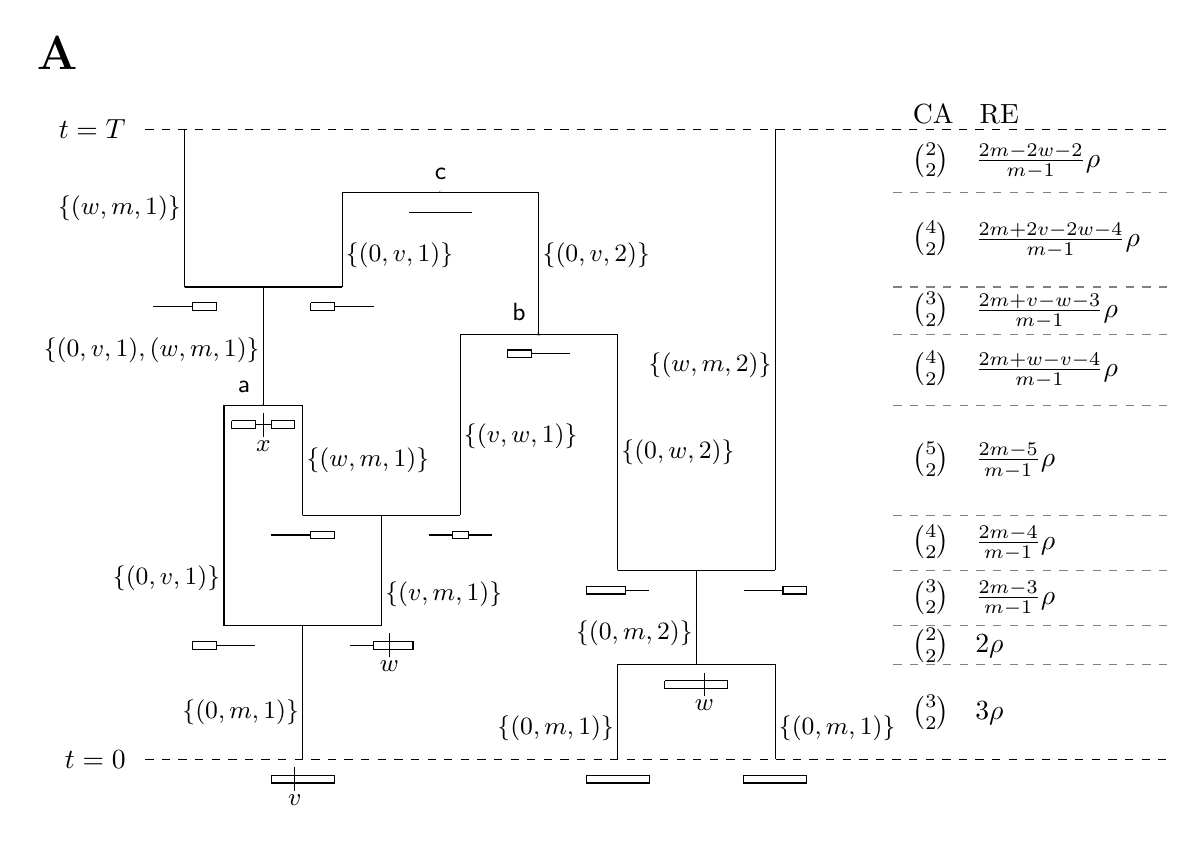
\begin{tikzpicture}
	\node [anchor=north west] at (-3.5,9.3) {\LARGE \textbf{A}};
	\draw (-0.4, -0.2) -- (0.4, -0.2) -- (0.4, -0.3) -- (-0.4, -0.3) -- (-0.4, -0.2);
	\draw (-0.1, -0.1) -- (-0.1, -0.4);
	\node [label=below:{\small $v$}] at (-0.1, -0.2) {};
	\draw (3.6, -0.2) -- (4.4, -0.2) -- (4.4, -0.3) -- (3.6, -0.3) -- (3.6, -0.2);
	\draw (5.6, -0.2) -- (6.4, -0.2) -- (6.4, -0.3) -- (5.6, -0.3) -- (5.6, -0.2);

	\draw (4,0) -- (4, 1.2) -- (6, 1.2) -- (6,0);
	\draw (4.6, 1) -- (5.4, 1) -- (5.4, 0.9) -- (4.6, 0.9) -- (4.6, 1);
	\draw (5.1, 1.1) -- (5.1, 0.8);
	\node [label=below:{\small $w$}] at (5.1, 1) {};

	\draw (0, 0) -- (0, 1.7) -- (-1,1.7) -- (1,1.7);
	\draw (-1.4, 1.5) -- (-1.1, 1.5) -- (-1.1, 1.4) -- (-1.4, 1.4) -- (-1.4, 1.5);
	\draw (-1.1, 1.45) -- (-0.6, 1.45);
	\draw (0.6, 1.45) -- (0.9, 1.45);
	\draw (0.9, 1.5) -- (1.4, 1.5) -- (1.4, 1.4) -- (0.9, 1.4) -- (0.9, 1.5);
	\draw (1.1, 1.6) -- (1.1, 1.3);
	\node [label=below:{\small $w$}] at (1.1, 1.5) {};

	\draw (5, 1.2) -- (5, 2.4) -- (4,2.4) -- (6,2.4);
	\draw (3.6, 2.2) -- (4.1, 2.2) -- (4.1, 2.1) -- (3.6, 2.1) -- (3.6, 2.2);
	\draw (4.1, 2.15) -- (4.4, 2.15);
	\draw (5.6, 2.15) -- (6.1, 2.15);
	\draw (6.1, 2.2) -- (6.4, 2.2) -- (6.4, 2.1) -- (6.1, 2.1) -- (6.1, 2.2);

	\draw (1, 1.7) -- (1, 3.1) -- (0,3.1) -- (2,3.1);
	\draw (-0.4, 2.85) -- (0.1, 2.85);
	\draw (0.1, 2.9) -- (0.4, 2.9) -- (0.4, 2.8) -- (0.1, 2.8) -- (0.1, 2.9);
	\draw (1.6, 2.85) -- (1.9, 2.85);
	\draw (1.9, 2.9) -- (2.1, 2.9) -- (2.1, 2.8) -- (1.9, 2.8) -- (1.9, 2.9);
	\draw (2.1, 2.85) -- (2.4, 2.85);

	\draw (-1, 1.7) -- (-1, 4.5) -- (0,4.5) -- (0,3.1);
	\node [scale=0.2,label=above left:{\small \noderef{a}}] at (-0.5,4.5) {a};
	\draw (-0.9, 4.3) -- (-0.6, 4.3) -- (-0.6, 4.2) -- (-0.9, 4.2) -- (-0.9, 4.3);
	\draw (-0.6, 4.25) -- (-0.4, 4.25);
	\draw (-0.4, 4.3) -- (-0.1, 4.3) -- (-0.1, 4.2) -- (-0.4, 4.2) -- (-0.4, 4.3);
	\draw (-0.5, 4.4) -- (-0.5, 4.1);
	\node [label=below:{\small $x$}] at (-0.5, 4.3) {};

	\draw (4,2.4) -- (4,5.4) -- (2,5.4) -- (2,3.1);
	\node [scale=0.2,label=above left:{\small \noderef{b}}] at (3,5.4) {b};
	\draw (2.6, 5.2) -- (2.9, 5.2) -- (2.9, 5.1) -- (2.6, 5.1) -- (2.6, 5.2);
	\draw (2.9, 5.15) -- (3.4, 5.15);

	\draw (-0.5, 4.5) -- (-0.5, 6) -- (-1.5,6) -- (0.5,6);
	\draw (-1.9, 5.75) -- (-1.4, 5.75);
	\draw (-1.4, 5.8) -- (-1.1, 5.8) -- (-1.1, 5.7) -- (-1.4, 5.7) -- (-1.4, 5.8);
	\draw (0.1, 5.8) -- (0.4, 5.8) -- (0.4, 5.7) -- (0.1, 5.7) -- (0.1, 5.8);
	\draw (0.4, 5.75) -- (0.9, 5.75);

	\draw (0.5, 6) -- (0.5, 7.2) -- (3,7.2) -- (3,5.4);
	\node [scale=0.2,label=above:{\small \noderef{c}}] at (1.75,7.2) {c};
	\draw (1.35, 6.95) -- (2.15, 6.95);

	\draw (-1.5, 6) -- (-1.5, 8);
	\draw (6, 2.4) -- (6, 8);

	% Edge annotations above each event
	\node [label=left:{\small$\{(0,m,1)\}$}] at (0.2,0.6) {};
	\node [label=left:{\small$\{(0,m,1)\}$}] at (4.2,0.4) {};
	\node [label=right:{\small$\{(0,m,1)\}$}] at (5.8,0.4) {};
	\node [label=left:{\small$\{(0,m,2)\}$}] at (5.2,1.6) {};
	\node [label=left:{\small$\{(0,v,1)\}$}] at (-0.8,2.3) {};
	\node [label=right:{\small$\{(v,m,1)\}$}] at (0.8,2.1) {};
	\node [label=right:{\small$\{(0,w,2)\}$}] at (3.8,3.9) {};
	\node [label=left:{\small$\{(w,m,2)\}$}] at (6.2,5) {};
	\node [label=right:{\small$\{(w,m,1)\}$}] at (-0.2,3.8) {};
	\node [label=right:{\small$\{(v,w,1)\}$}] at (1.8,4.1) {};
	\node [label=left:{\small$\{(0,v,1), (w,m,1)\}$}] at (-0.3,5.2) {};
	\node [label=right:{\small$\{(0,v,2)\}$}] at (2.8,6.4) {};
	\node [label=left:{\small$\{(w,m,1)\}$}] at (-1.3,7) {};
	\node [label=right:{\small$\{(0,v,1)\}$}] at (0.3,6.4) {};

	% Dashed lines for start and end times
	\draw[dashed] (-2, 0) -- (11, 0);
	\node [label=left:{$t = 0$}] at (-2,0) {};
	\draw[dashed] (-2, 8) -- (11, 8);
	\node [label=left:{$t = T$}] at (-2,8) {};

	% Numbers of extant ancestors and links, from top to bottom
	\node[label=right:{CA \; RE}] at (7.5, 8.2) {};
	\node[label=right:{$\binom{2}{2}$ \; $\frac{2 m - 2 w - 2}{m - 1} \rho$}] at (7.5, 7.6) {};
	\node[label=right:{$\binom{4}{2}$ \; $\frac{2 m + 2 v - 2 w - 4}{m - 1} \rho$}] at (7.5, 6.6) {};
	\node[label=right:{$\binom{3}{2}$ \; $\frac{2 m + v - w - 3}{m - 1} \rho$}] at (7.5, 5.7) {};
	\node[label=right:{$\binom{4}{2}$ \; $\frac{2 m + w - v - 4}{m - 1} \rho$}] at (7.5, 4.95) {};
	\node[label=right:{$\binom{5}{2}$ \; $\frac{2 m - 5}{m - 1} \rho$}] at (7.5, 3.8) {};
	\node[label=right:{$\binom{4}{2}$ \; $\frac{2 m - 4}{m -1} \rho$}] at (7.5, 2.75) {};
	\node[label=right:{$\binom{3}{2}$ \; $\frac{2 m - 3}{m - 1} \rho$}] at (7.5, 2.05) {};
	\node[label=right:{$\binom{2}{2}$ \; $2 \rho$}] at (7.5, 1.45) {};
	\node[label=right:{$\binom{3}{2}$ \; $3 \rho$}] at (7.5, 0.6) {};

	% Gray dashed lines to visually separate holding times
	\draw[color=gray, dashed] (7.5, 1.2) -- (11, 1.2);
	\draw[color=gray, dashed] (7.5, 1.7) -- (11, 1.7);
	\draw[color=gray, dashed] (7.5, 2.4) -- (11, 2.4);
	\draw[color=gray, dashed] (7.5, 3.1) -- (11, 3.1);
	\draw[color=gray, dashed] (7.5, 4.5) -- (11, 4.5);
	\draw[color=gray, dashed] (7.5, 5.4) -- (11, 5.4);
	\draw[color=gray, dashed] (7.5, 6) -- (11, 6);
	\draw[color=gray, dashed] (7.5, 7.2) -- (11, 7.2);
\end{tikzpicture}
&
\begin{tikzpicture}
	\node [anchor=north west] at (-3.5,9.3) {\LARGE \textbf{B}};
	\draw (-0.4, -0.2) -- (0.4, -0.2) -- (0.4, -0.3) -- (-0.4, -0.3) -- (-0.4, -0.2);
	\draw (-0.1, -0.1) -- (-0.1, -0.4);
	\node [label=below:{\small $v$}] at (-0.1, -0.2) {};
	\draw (3.6, -0.2) -- (4.4, -0.2) -- (4.4, -0.3) -- (3.6, -0.3) -- (3.6, -0.2);
	\draw (5.6, -0.2) -- (6.4, -0.2) -- (6.4, -0.3) -- (5.6, -0.3) -- (5.6, -0.2);

	\draw (4,0) -- (4, 1.2) -- (6, 1.2) -- (6,0);
	\draw (4.6, 1) -- (5.4, 1) -- (5.4, 0.9) -- (4.6, 0.9) -- (4.6, 1);
	\draw (5.1, 1.1) -- (5.1, 0.8);
	\node [label=below:{\small $w$}] at (5.1, 1) {};

	\draw (0, 0) -- (0, 1.7) -- (-1,1.7) -- (1,1.7);
	\draw (-1.4, 1.5) -- (-1.1, 1.5) -- (-1.1, 1.4) -- (-1.4, 1.4) -- (-1.4, 1.5);
	\draw (-1.1, 1.45) -- (-0.6, 1.45);
	\draw (0.6, 1.45) -- (0.9, 1.45);
	\draw (0.9, 1.5) -- (1.4, 1.5) -- (1.4, 1.4) -- (0.9, 1.4) -- (0.9, 1.5);
	\draw (1.1, 1.6) -- (1.1, 1.3);
	\node [label=below:{\small $w$}] at (1.1, 1.5) {};

	\draw (5, 1.2) -- (5, 2.4) -- (4,2.4) -- (6,2.4);
	\draw (3.6, 2.2) -- (4.1, 2.2) -- (4.1, 2.1) -- (3.6, 2.1) -- (3.6, 2.2);
	\draw (4.1, 2.15) -- (4.4, 2.15);
	\draw (5.6, 2.15) -- (6.1, 2.15);
	\draw (6.1, 2.2) -- (6.4, 2.2) -- (6.4, 2.1) -- (6.1, 2.1) -- (6.1, 2.2);
	\draw [color=red](5.8, 2.3) -- (5.8, 2.0);
	\node [label={[red]below:{\small $y$}}] at (5.8, 2.1) {};

	\draw (1, 1.7) -- (1, 3.1) -- (0,3.1) -- (2,3.1);
	\draw (-0.4, 2.85) -- (0.1, 2.85);
	\draw (0.1, 2.9) -- (0.4, 2.9) -- (0.4, 2.8) -- (0.1, 2.8) -- (0.1, 2.9);
	\draw (1.6, 2.85) -- (1.9, 2.85);
	\draw (1.9, 2.9) -- (2.1, 2.9) -- (2.1, 2.8) -- (1.9, 2.8) -- (1.9, 2.9);
	\draw (2.1, 2.85) -- (2.4, 2.85);

	\draw (-1, 1.7) -- (-1, 4.5) -- (0,4.5) -- (0,3.1);
	\draw (-0.9, 4.3) -- (-0.6, 4.3) -- (-0.6, 4.2) -- (-0.9, 4.2) -- (-0.9, 4.3);
	\draw (-0.6, 4.25) -- (-0.4, 4.25);
	\draw (-0.4, 4.3) -- (-0.1, 4.3) -- (-0.1, 4.2) -- (-0.4, 4.2) -- (-0.4, 4.3);
	\draw (-0.5, 4.4) -- (-0.5, 4.1);
	\node [label=below:{\small $x$}] at (-0.5, 4.3) {};

	\draw (6, 2.4) -- (6, 3.8) -- (7, 3.8);
	\draw [color=red](6, 3.8) -- (5, 3.8);
	\draw (4.6, 3.55) -- (5.4, 3.55);
	\draw (6.6, 3.55) -- (7.1, 3.55);
	\draw (7.1, 3.6) -- (7.4, 3.6) -- (7.4, 3.5) -- (7.1, 3.5) -- (7.1, 3.6);

	\draw (4,2.4) -- (4,5.4) -- (2,5.4) -- (2,3.1);
	\draw (2.6, 5.2) -- (2.9, 5.2) -- (2.9, 5.1) -- (2.6, 5.1) -- (2.6, 5.2);
	\draw (2.9, 5.15) -- (3.4, 5.15);

	\draw (-0.5, 4.5) -- (-0.5, 6) -- (-1.5,6) -- (0.5,6);
	\draw (-1.9, 5.75) -- (-1.4, 5.75);
	\draw (-1.4, 5.8) -- (-1.1, 5.8) -- (-1.1, 5.7) -- (-1.4, 5.7) -- (-1.4, 5.8);
	\draw (0.1, 5.8) -- (0.4, 5.8) -- (0.4, 5.7) -- (0.1, 5.7) -- (0.1, 5.8);
	\draw (0.4, 5.75) -- (0.9, 5.75);

	\draw [color=red](5, 3.8) -- (5, 6.6) -- (4, 6.6);
	\draw (4,6.6) -- (3,6.6) -- (3, 5.4);
	\draw (3.6, 6.4) -- (3.9, 6.4) -- (3.9, 6.3) -- (3.6, 6.3) -- (3.6, 6.4);
	\draw (3.9, 6.35) -- (4.4, 6.35);

	\draw (0.5, 6) -- (0.5, 7.2) -- (4,7.2) -- (4,6.6);
	\draw (1.85, 6.95) -- (2.65, 6.95);

	\draw (-1.5, 6) -- (-1.5, 8);
	\draw [color=red](2.25, 7.2) -- (2.25, 8);
	\draw (7, 3.8) -- (7, 8);

	% Dashed lines for start and end times
	\draw[dashed] (-2, 0) -- (9.1, 0);
	\node [label=left:{$t = 0$}] at (-2,0) {};
	\draw[dashed] (-2, 8) -- (9.1, 8);
	\node [label=left:{$t = T$}] at (-2,8) {};

	% Numbers of extant ancestors and links, from top to bottom
	\node[label=right:{CA \; RE}] at (7.5, 8.2) {};
	\node[label=right:{$\binom{3}{2}$ \; $3 \rho$}] at (7.5, 7.6) {};
	\node[label=right:{$\binom{4}{2}$ \; $4 \rho$}] at (7.5, 6.9) {};
	\node[label=right:{$\binom{5}{2}$ \; $5 \rho$}] at (7.5, 6.3) {};
	\node[label=right:{$\binom{4}{2}$ \; $4 \rho$}] at (7.5, 5.7) {};
	\node[label=right:{$\binom{5}{2}$ \; $5 \rho$}] at (7.5, 4.95) {};
	\node[label=right:{$\binom{6}{2}$ \; $6 \rho$}] at (7.5, 4.15) {};
	\node[label=right:{$\binom{5}{2}$ \; $5 \rho$}] at (7.5, 3.45) {};
	\node[label=right:{$\binom{4}{2}$ \; $4 \rho$}] at (7.5, 2.75) {};
	\node[label=right:{$\binom{3}{2}$ \; $3 \rho$}] at (7.5, 2.05) {};
	\node[label=right:{$\binom{2}{2}$ \; $2 \rho$}] at (7.5, 1.45) {};
	\node[label=right:{$\binom{3}{2}$ \; $3 \rho$}] at (7.5, 0.6) {};

	% Gray dashed lines to visually separate holding times
	\draw[color=gray, dashed] (7.5, 1.2) -- (9.1, 1.2);
	\draw[color=gray, dashed] (7.5, 1.7) -- (9.1, 1.7);
	\draw[color=gray, dashed] (7.5, 2.4) -- (9.1, 2.4);
	\draw[color=gray, dashed] (7.5, 3.1) -- (9.1, 3.1);
	\draw[color=gray, dashed] (7.5, 3.8) -- (9.1, 3.8);
	\draw[color=gray, dashed] (7.5, 4.5) -- (9.1, 4.5);
	\draw[color=gray, dashed] (7.5, 5.4) -- (9.1, 5.4);
	\draw[color=gray, dashed] (7.5, 6) -- (9.1, 6);
	\draw[color=gray, dashed] (7.5, 6.6) -- (9.1, 6.6);
	\draw[color=gray, dashed] (7.5, 7.2) -- (9.1, 7.2);
\end{tikzpicture}
\end{tabular}
}
\caption{(A)
A realisation of the graph traversed by Hudson's algorithm started from a
sample of three chromosomes with $m$ discrete sites each at time $t = 0$, and
propagated until time $T$. The MRCA on the genetic interval $[v, w)$ is reached
at event \noderef{b}, while that on $[0, v)$ is reached at event \noderef{c}.
The non-ancestral segment $[v, w)$ above
\noderef{a} contributes to the rate of effective recombinations because it
is trapped between ancestral segments. The two columns titled CA and RE
are the respective rates of mergers and recombinations when
the recombination rate is $\rho$.
(B) A corresponding realisation of a Big ARG, which augments Hudson's algorithm
by tracking non-ancestral lineages. The result is a simpler state space and
dynamics, at the cost of extra nodes and edges, highlighted in red, which do
not affect the local tree at any site.
Recombination positions are labelled alphabetically in time, and their ordering
along the genome is $y < v < x < w$, of which the first only appears in panel B.
There are two separate recombination events at link $w$.
}
\label{hudson_vs_bigARG}
\end{figure}

Figure \ref{hudson_vs_bigARG} illustrates the more complex state space
of the Little ARG process, as well as the extra events which occur in the Big ARG process.
Moreover, it depicts the rates of common ancestors and recombination events in each
interval of time of the realisations.
In order to evaluate these rates, e.g.\ for likelihood-based inference
\citep{baumdicker2021efficient, mahmoudi2022bayesian},
it is necessary to know the number of lineages and number of extant links
available for recombination in each time interval.
Some representations may not provide this information.
For example, in the gARG encoding depicted in Figure \ref{fig-ancestry-resolution}C,
it is clear that a recombination takes place between nodes \noderef{i}, \noderef{k} and \noderef{j}.
But the exact time of the recombination event is ambiguous: it could take place at any time between node \noderef{i} and its parents and produce the same gARG.
Because a recombination increases the number of extant lineages by one (in the rootward direction of time), the number of lineages during the same time interval is ambiguous as well.
In fact, this information cannot be recovered from the gARG encoding used in Figure \ref{fig-ancestry-resolution}C without an extrinsic convention.
For the basic coalescent with recombination,
it is sufficient to create \emph{two} gARG nodes at the time of the recombination event, with the interpretation that the two rootward edges from node \noderef{i} in Figure \ref{fig-ancestry-resolution}C belong to the same lineage until the time of nodes \noderef{k} and \noderef{j}, and split into two separate lineages at that time point.
Similarly, the trapped, non-ancestral links along that lineage remain available for effective recombination (i.e.\ one which splits up ancestral material) for the same time interval.
This interpretation is highlighted in
Figure \ref{hudson_vs_bigARG} by drawing only one vertical edge between a recombinant child and its two parents.


% Full quote:
% This process simplifies mathematics on the account that the notion of an
% ancestor will have a less restrictive meaning than usual:
% An ``ancestral'' sequence in the birth and death process
% need not have any genetic material in common with a
% sequence descended from it.

\section{Survey of ARG inference methods}
\label{sec-survey-arg-infer}

The problem of reconstructing ARGs for samples of recombining sequences has
been of interest since the ARG was first defined. Early methods focused on
finding \emph{parsimonious} ARGs, i.e.\ those with a minimal number of
recombination events~\citep{hein1990reconstructing}. Two main approaches
emerged: ``backwards-in-time''~\citep{lyngso2005minimum} and
``along-the-genome'' \citep{song2003parsimonious, song2005constructing}.
Backwards-in-time approaches
start with a data matrix and reduce it to an empty matrix through row
and column operations corresponding to coalescence, mutation, and recombination
events, which construct an ARG from the bottom up~\citep{song2005efficient,
wu2008association,thao2019hybrid,ignatieva2021kwarg}.
Along-the-genome approaches
begin from an initial local tree at a single focal site.
Moving the focal site along the
genome changes the local tree via a subtree prune and regraft
operation whenever a recombination is encountered~\citep{hein1993heuristic,
wu2011new, mirzaei2017rent}.
\citet{rasmussen2022espalier} focus on parsimonious fusion of local
trees into an ARG, while the method described by
\citet{camara2016inference} is based on topological data analysis.
% The "most" is understood here, surely
Reconstructing a parsimonious ARG for a given data set is NP-hard
\citep{wang2001perfect}, so parsimony-based methods resort to heuristics and
are limited to analysing at most hundreds of sequences. Hence, a number of
methods aim to balance computational efficiency with reconstruction of
``reasonable'', rather than parsimonious ARGs
% distribution under a population genetics model
\citep{minichiello2006mapping,
parida2008estimating, kelleher2019inferring,  speidel2019method,
schaefer2021ancestral, zhang2023biobank}.

% AI: just to note, these papers do not all agree in their definition of an
% ARG. I guess this is one of the points of the present paper, but should we
% mention this fact? Should we also mention that most of these infer just the
% topology, but some also the times?

An alternative approach is to treat the ARG as a latent parameter to be
averaged out by Monte Carlo methods, based either on importance sampling
\citep{griffiths1996ancestral, fearnhead2001estimating, jenkins2011inference}
or MCMC \citep{kuhner2000maximum, kuhner2006lamarc, nielsen2000estimation, wang2008bayesian,
wang2009population, fallon2013acg, vaughan2017inferring, mahmoudi2022bayesian}.
These methods operate on representations
of the ``Little ARG'' (see Appendix \ref{sec-big-and-little-arg}), and are computationally expensive, being
applicable to at most hundreds of samples consisting of tens or hundreds of
kilobases with human-like parameters.
State-of-the-art methods rely on cheaper,
approximate models \citep{didelot2010inference, heine2018bridging,
hubisz2020mapping,hubisz2020inference, medina2020speeding}. The most scalable
method, \texttt{ARGWeaver} \citep{rasmussen2014genome}, can be applied to
dozens of mammal-like genomes \citep{hubisz2020inference}.

Methods to sample ARGs generate a ``cloud'' of estimates, and
\cite{kuhner2017consensus} provide an approach to generate a
set of consensus breakpoints and local trees from
such a cloud.
The approach is based on examining the recombination breakpoints
in all of the input ARGS, and including those that are
in at least $k$ of the input ARGs (with some additional
filtering criteria) in the output.
Within the resulting intervals, a consensus
local tree is then generated using standard phylogenetic methods.

% Not sure we want this content now? We're not really talking about
% evaluation of liklihoods any more.
% A central quantity
% in all of these sampling methods is the conditional sampling probability $p(G |
% D) \propto p(D | G) p(G)$ of an ARG $G$ given an observed realization of
% genetic diversity $D$ at its sampled leaves, where $p(D | G)$ is the likelihood
% of the data $D$ given $G$, and $p(G)$ is a Bayesian prior distribution or a
% frequentist regularizer for the ARG $G$.

% The likelihood $p(D | G)$ is effectively always the distribution of a Poisson
% process on the ancestral material along the edges of $G$ \citep[Eq.\
% (2)]{mahmoudi2022bayesian}. Hence it is typically straightforward to evaluate
% in principle, but choosing the right data structure can still have a dramatic
% effect on the efficiency of evaluation \citep{mahmoudi2022bayesian}. Especially
% in the Bayesian case, $p(G)$ is typically specified as the sampling
% distribution of a stochastic process, such as the coalescent with
% recombination. Two contemporary examples are \citet{mahmoudi2022bayesian} and
% \citet{guo2022recombination}. Evaluating the distribution of the coalescent with
% recombination (or related models) requires knowledge of the number of extant
% lineages and number of links available for recombination (i.e.\ ones at which a
% recombination would split ancestral material) at each time \citep[Eq.\
% (3)]{mahmoudi2022bayesian}. These require a data structure from which shared
% edges on different trees are easy to identify, and which encodes recombination
% events and times explicitly, e.g.\ using nodes.

\section{Cell lineages and ARGs}
\label{sec-cell-lineages-and-args}
\begin{figure}
\begin{center}
    \includegraphics[width=0.8\textwidth]{illustrations/cell-lines}
\end{center}
\caption{\label{fig-cell-lines}
Cellular inheritance of a single chromosome in a diploid population.
Individuals (blue) contain diploid cells (white circles enclosing a homologous pair of chromosomes).
For clarity, only two rounds of mitotic germ-line cell division are shown per individual, and
meiosis is not illustrated in detail.
Lines show prospective inheritance paths for all chromosomes. Solid lines show all possible
retrospective ancestry paths for four chosen chromosomes (indicated by square black ``sampling events'')
sampled from 3 diploid individuals ($D_1$, $D_2$, $D_3$) in the current generation.
Ancestral recombination events and coalescence events are shown as red and blue squares respectively.
A realised ARG path for the lower arm of the sampled chromosomes is highlighted as a
thick solid line, passing through a set of potential gARG nodes (green). This ARG
involves a single recombination event and four coalescence events
(highlighted as deep red and blue squares within individuals $D_5$, $D_{10}$, and $D_{13}$).
ARG lineages also show gametic genomes, contained within shaded circles.
As in Fig.~\ref{fig-arg-in-pedigree}A, inherited regions within the sampled chromosome arm are
shaded by the number of descendant samples.
}
\end{figure}

In eukaryotes, ARGs are a result of the cellular processes of mitosis and meiosis.
Mitosis leads to common ancestor events,
and meiosis leads to recombination events (both crossover and gene conversion).
Fig.~\ref{fig-simplification} shows a schematic of the events  and
the genomes (chromosome icons) that occur in the cellular
germline of a simplified, diploid multicellular
hermaphrodite eukaryote with partially overlapping generations.
Here, an event is not represented by a specific
genome. Rather, genomes can be associated with, or ``tag'', events above
(ancestral to) or below (descended from) them.
For example, tagging the two genomes above a recombination event leads to the
two node representation seen in
Figs.~\ref{fig-simplification} and \ref{hudson_vs_bigARG},
whereas tagging the genome
below a recombination event leads to the more
conventional graphs in Figs.~\ref{fig-ancestry-resolution} and \ref{fig-inferred-args}A,B.

%% JK:  What does this add that is not in caption?
% Thick black lines trace an ARG that describes the ancestry of the lower arm of
% the four sampled chromosomes, and these lines pass through gARG nodes (green
% chromosomal regions). A number of these nodes have only one parent and one
% child in the ARG; these would often be omitted (taken as implicit) in a
% minimally simplified gARG.

The schematic illustrates an important point about the biological reality of polytomies.
Three linages coalesce in the left-hand genome of individual $D_{10}$, but do
so as the result of two successive bifurcations. This is \emph{necessarily} so,
because the only known method of reproducing DNA is by (semi-conservative) duplication.
Whether this polytomy is resolvable depends on the available mutational data.
Mutations can occur along any cell lineages. For example,
a mutation in the first cell division of $D_{10}$ could be shared between
the two gametes produced by the cells in the left half of $D_{10}$
but not shared by the right hand gamete.
With enough mutations, each
round of mitotic germline genome duplication within a single multicellular organism could
in principle be distinguished.

% Note that mutations can occur along any lineage in Fig.~\ref{fig-cell-lines}. This means, for example,
% that a mutation in the first cell division of $D_{10}$ could be shared between
% the two gametes produced by the cells in the left half of $D_{10}$ but not shared by
% the right hand gamete. With a high enough mutation rate (or equivalently, a long enough genome), each
% round of mitotic germline genome duplication within a single multicellular organism could
% potentially be distinguished.
% This implies that in ARGs that have been inferred from real data, polytomies represent a lack
% of mutational information (rather than marking a single ``multifurcation event'').
% The ability to represent polytomies, and conceptualise them as a (deliberately) imprecise statement about the order
% of coalescence within and between individuals,
% fits naturally into the gARG framework presented in this paper.

\clearpage
\renewcommand\thefigure{S\arabic{figure}}
\setcounter{figure}{0}
\renewcommand\thetable{S\arabic{table}}
\setcounter{table}{0}

\section*{Supplementary Material}

\begin{figure}[ht]
	\begin{center}
		\includegraphics[width=0.8\textwidth]{illustrations/simplification-with-edges.pdf}
	\end{center}
	\caption{\label{fig-simplification-with-edges}
	Example ARGs Fig.~\ref{fig-simplification}A--D,
    with edges annotated with inheritance intervals.
	}
\end{figure}

\end{document}
